%% =========================================================================
%% Manuscript for the Journal of Building Engineering (Elsevier)
%% Class: elsarticle (vendored in this folder — no TeX package install needed;
%%        also works as-is on Overleaf: upload the whole manuscript/ folder)
%%
%% Compile:  pdflatex main && bibtex main && pdflatex main && pdflatex main
%%
%% Class options:
%%   [review]   — double line spacing + line numbers (use for SUBMISSION)
%%   [preprint] — single spacing, no line numbers (use for internal drafts)
%%   [5p,twocolumn] — approximates final journal layout (for length checks)
%%
%% STRUCTURE (2026-07-11): main.tex holds only the preamble, front matter,
%% and bibliography; each section lives in its own file under sections/ and
%% is pulled in with \input below. Edit the section files, not this one, for
%% prose changes.
%%
%% OUTLINE DRAFT — structure + the parts writable before the analysis
%% results exist. Sources: the team's planning docs
%% (bbr-demolitions/docs/plan.md, indicators.md, indicator-decision.md),
%% the verified BBR code lists, and the published papers on file.
%% No analytical conclusions are drawn in this draft; those are written by
%% the group once results/ is populated.
%%
%% Marker legend (all colored, all must be gone before submission):
%%   \pending{...}       orange — awaiting the analysis run (Linus & Oscar)
%%   \groupdecision{...} purple — open decision for the whole group
%%   \refneeded{...}     red    — claim needs a verified reference
%%   \slotfor{...}{...}  blue   — section/paragraph reserved for Rune/Nicolai
%%   \draftnote{...}     gray   — note to co-authors about the draft itself
%% =========================================================================
\documentclass[preprint,12pt]{elsarticle}

\usepackage{graphicx}
\usepackage{subcaption}
\usepackage{booktabs}
\usepackage{array}
\usepackage{amsmath}
\usepackage{xcolor}
\usepackage[hidelinks]{hyperref}
\usepackage{tikz}
\usetikzlibrary{arrows.meta,positioning,calc}
\usepackage{float} % enables [H] to pin the indicator schematics in place

% ---- Draft-status markers (remove before submission) --------------------
\newcommand{\pending}[1]{\textcolor{orange!85!black}{\textbf{[PENDING:} #1\textbf{]}}}
\newcommand{\groupdecision}[1]{\textcolor{violet}{\textbf{[GROUP DECISION:} #1\textbf{]}}}
\newcommand{\refneeded}[1]{\textcolor{red}{\textbf{[REF:} #1\textbf{]}}}
\newcommand{\slotfor}[2]{\begin{quote}\color{blue!65!black}\itshape\textbf{[SLOT --- #1]} #2\end{quote}}
\newcommand{\draftnote}[1]{\begin{quote}\color{gray}\small\itshape #1\end{quote}}

% ---- Style for the indicator-mechanism schematics (Section~\ref{sec:ind-mechanisms}) ----
\tikzset{
  ind/.style={draw, thick, rounded corners, align=center, text width=5.3cm,
              minimum height=0.65cm, inner sep=4pt, font=\footnotesize},
  indnote/.style={font=\scriptsize\itshape, align=left, text width=4.0cm},
  indarrow/.style={-{Latex[length=2.2mm]}, thick}
}

% Journal name for the footer of the title page
\journal{Journal of Building Engineering}

\begin{document}

\begin{frontmatter}

%% TODO: working title — refine with the group
\title{Sensitivity of national building demolition statistics to
       register-based indicator and floor-area assumptions:
       evidence from the Danish Building and Housing Register}

%% Authors and affiliations.
%% TODO: decide author order, corresponding author; Rune and Nicolai
%%       expected as co-authors per the agreed writing split (JOBE: no
%%       authorship changes after acceptance!). Affiliations to be added.
\author[dtu]{Theodor Dornonville de la Cour}
\author[dtu]{Linus Juni}
\author[dtu]{Oscar Johan H{\o}eg Wohlfahrt}
\author[dtu]{Nicolai Siim Larsen}
\author[dtu]{Rune Andersen}
%\author[dtu]{Nicolai Siim Larsen}   % TODO: confirm authorship + affiliation
%\author[dtu2]{Rune Andersen}        % TODO: confirm authorship + affiliation

\affiliation[dtu]{organization={Technical University of Denmark, Department of Applied Mathematics and Computer Science},
                  addressline={Richard Petersens Plads, Building 324},
                  city={Kgs.\ Lyngby},
                  postcode={2800},
                  country={Denmark}}
%\affiliation[dtu2]{organization={Technical University of Denmark, Department of Environmental and Resource Engineering},
%                  city={Kgs.\ Lyngby}, postcode={2800}, country={Denmark}}

%% TODO: abstract, max 250 words, standalone, no undefined abbreviations,
%%       no citations. To be written by the group once results exist.
\begin{abstract}
[TODO: 2--3 sentences on purpose: demolition estimates from the Danish
Building and Housing Register (BBR) depend on how ``a demolition'' and
``floor area'' are operationalized; this study quantifies that
sensitivity.]
[TODO: 2--3 sentences on method: the same demolition-rate computation
repeated under each candidate demolition indicator crossed with each
candidate floor-area measure, on a complete BBR extract (including
historical records) through 2025.]
[TODO: principal quantitative result: the spread across scenarios.]
[TODO: comparison with published BUILD figures.]
[TODO: main conclusion and recommendation --- \emph{to be decided by the
group from the results}.]
\end{abstract}

%% 1-7 keywords, no "and"/"of" constructions
\begin{keyword}
Building demolition \sep Building stock \sep Service life \sep
Building register \sep Data quality \sep Denmark
\end{keyword}

\end{frontmatter}

%% =========================================================================
%% Section files (edit these for prose changes).
%% =========================================================================
%% =========================================================================
\section{Introduction}\label{sec:intro}

\draftnote{Full draft (2026-07-12), written in plain language. Structure:
P1 why demolition data matters; P2 prior estimates and the indicator behind
each; P3 the problem (BBR has no clean demolition flag); P4 the gap and the
novelty; P5 objectives; P6 short road map. Related work is folded in here
(P2, P4) rather than in a separate section. Remaining markers: \pending{}
for the one headline number the group confirms from results, and
\refneeded{} for the Danish mandatory-LCA citation. RUNE/NICOLAI: please
review and, if useful, add one or two more international references to P2.}

%% ---- P1: why demolition rates matter ------------------------------------
The building sector has a large environmental footprint. Buildings and
their construction account for about a third of the world's energy use and
of its energy-related carbon emissions, and the materials used to build
them cause roughly a further one-fifth of global emissions on their
own~\cite{unep2025gsr}. When a building is demolished, some of its
materials can be recycled or reused, but in practice recovered materials
cover only a small part of what new construction
needs~\cite{andersen2022adaptation}, so much of the carbon already invested
in the building is still lost and new construction is needed to replace
it -- which is why replacing a building generally carries a higher climate
impact than keeping it~\cite{huuhka2023renovate}. How long buildings last, and how many are torn down
each year, therefore matters for several kinds of building-engineering
work. Whole-building life cycle assessment (LCA) uses an assumed building
service life to decide how many times components are replaced and how the
results are reported over time~\cite{ostergaard2018temporal,iso15686}; this
assumption strongly affects the calculated environmental
impact~\cite{andersen2023lifespan}. In Denmark this is no longer only an
academic concern: since 2023 the building regulations require an LCA for
new buildings, calculated over a fixed 50-year period that is set for
comparability rather than to match any building's real
lifespan~\cite{br18_klima}. Models of the building stock and of material flows
also need to know how much is demolished, because demolition is the flow
that leaves the stock and that supplies materials for
reuse~\cite{negendahl2022parametric,andersen2022adaptation}.

%% ---- P2: prior Danish estimates and the indicator behind each -----------
Published estimates of how much is demolished in Denmark, and of how long
Danish buildings last, differ widely. For Denmark alone, reported building
service lives run from medians near 55~years~\cite{ostergaard2018temporal}
to the 120~years assumed in the standard service-life
tables~\cite{aagaard2013levetider}. A key reason is that each study measures
demolition in a different way, even though they draw on the same source: the
Danish Building and Housing Register (Bygnings- og Boligregistret, BBR). The standard Danish service-life tables assume an
overall demolition rate of about 0.3\,\% of the stock per year, taken from
construction-cost statistics rather than from records of individual
buildings~\cite{aagaard2013levetider}. BUILD (Aalborg University) counts
buildings that have been \emph{retired} (``udg{\aa}et'') from the register
and reports on average about 2.2~million~m\textsuperscript{2} of demolished
floor area per year in 2012--2023, again close to 0.3\,\% of the stock by
area~\cite{jensen2025nedrivning}. Studies of building service life instead
start from records of demolition \emph{cases}: one estimates a median life
of roughly 60~years for single-family houses from 124{,}096
cases~\cite{andersen2023lifespan}, and a more recent one finds an
area-weighted median life of 87~years for housing from 106{,}908
demolitions, identified from a demolition-related update to the building
record~\cite{droob2026servicelife}. An earlier study of the temporal scope
of building LCAs used an administrative BBR extract of buildings
``demolished 2009--2015'' without stating how the extract was
made~\cite{ostergaard2018temporal}. Other studies do not use a register
flag at all, and instead detect demolition indirectly, as a house that is
torn down and rebuilt on the same
plot~\cite{jensen2022enfamiliehuse,blv2023karakteristika}. The same pattern
appears abroad: register-based studies in Finland and in a set of European
and US cities (including Copenhagen) each define a demolition as a building
that is removed from, or no longer survives in, a register, rather than as
a directly observed physical event~\cite{huuhka2021stocks,berglundbrown2025lifetimes}.
In short, each of these approaches turns ``a demolition'' into a different
concrete rule -- a register exit, a demolition-coded update, a compiled list
of demolition cases, or a rebuild pattern -- and they also differ in which
of BBR's several floor-area figures they add up.

%% ---- P3: the problem — BBR has no clean demolition flag -----------------
This variety is not careless; it reflects a real limitation of the data. A
register like BBR records administrative objects and processes, not
directly observed physical events, so a change in the register is not the
same as a change on the ground~\cite{mit2021admindata,un2019registers}. BBR
was designed for administration, and property owners are responsible for
reporting changes. The register does contain a purpose-built field that
would mark a completed physical demolition, but that field is not included
in the public data distributed through the national data
portal~\cite{bbr_instruks,datafordeler_grunddatamodel}. What the public data
does contain is a general ``historical'' status that a building also reaches
for other reasons, such as error corrections, mergers, and
re-registrations. There is therefore no single field in the distributed
data that cleanly and only marks a demolition. Asked directly how to tell,
the register authority itself pointed us not to a definitive field but to
the building's lifecycle status -- a proxy. The quality of BBR has also
been found to be uneven: a national audit reported that the extent and
significance of the errors were not even known, and that quality varied
considerably between municipalities~\cite{rigsrevisionen_bbr}, and later
coverage estimated that a large share of single-family houses were recorded
with incorrect measurements~\cite{dr2023bbr}. Faced with this, every
researcher has to build their own \emph{indicator}: an observable register
event, chosen to stand in for a demolition. Because the register offers no
agreed choice, different practitioners choose differently, and this is a
major reason their published numbers do not agree.

%% ---- P4: the gap and the novelty ----------------------------------------
What has not been studied is how much this single choice actually matters.
Earlier sensitivity analyses in building-stock research have varied other
things: the assumed shape of the building-lifespan distribution inside a
material-flow model~\cite{miatto2017buildinglifespan}, or the data
\emph{source} the demolitions are drawn from~\cite{huuhka2021stocks}. To the
best of our knowledge, no study has instead held everything else
fixed -- the same register, the same period, the same calculation -- and
changed only the demolition indicator, in order to measure how much the
resulting national demolition figures move. The novelty of this work is to
make that comparison directly. We treat the choice of indicator as the one
thing we vary, and we ask: how sensitive are Denmark's demolition figures to
how a demolition is defined in BBR? Alongside this main question we ask
several smaller ones: how much do the indicators agree on which buildings
they select; which building types are most affected; what difference excluding
discontinued building-use codes makes; how much the choice
of floor-area figure changes the reported area; and how our transparent
indicators compare with the compiled national extract the field has relied
on.

%% ---- P5: objectives ------------------------------------------------------
Accordingly, this study pursues three objectives. First, to define a set of
demolition indicators directly from a complete BBR extract -- including the
full history of demolished buildings -- so that every step is documented and
can be reproduced, in contrast to the pre-made and undocumented extracts
used in earlier work~\cite{kurvinen2021modeling}. Second, to run the same
demolition-rate calculation once for each indicator, holding all other
choices fixed, and to report how far the results spread. Third, to compare
these results with published Danish figures and with the compiled national
extract, so the practical consequences of the choice are clear. We find that
the choice is not a minor technicality: across indicators the number of
buildings counted as demolished differs by about 4.4-fold, and the reported
demolished floor area depends further on which area figure is used and on
how complete that figure is.

%% ---- P6: road map (optional; keep short) --------------------------------
The remainder of this paper is organised as follows.
Section~\ref{sec:bbr} describes BBR and how a demolition appears in it.
Section~\ref{sec:indicators} defines the demolition indicators we compare.
Section~\ref{sec:methods} explains the data and the shared calculation.
Section~\ref{sec:results} reports the results, and
Sections~\ref{sec:discussion} and~\ref{sec:conclusion} discuss them and
conclude.

%% =========================================================================
\section{The Danish Building and Housing Register (BBR)}\label{sec:bbr}

\draftnote{This section is descriptive and drafted in full: it renders
the register facts we verified against the official BBR code lists, the
grunddata object model, and the BBR case-processing instructions
(docs/indicator-decision.md and docs/indicators.md), plus the published
BUILD reports. Please check the wording against the sources; nothing
here should be new analysis.}

\subsection{Purpose, structure, and distribution}\label{sec:bbr-structure}

The Danish Building and Housing Register (Bygnings- og Boligregistret,
BBR) is the national administrative register of buildings and dwellings,
established by the Building and Housing Registration Act of 1976
(BBR-loven)~\cite{bbrloven}. It is maintained by the municipalities, and
%% NOTE: the register became operational/was populated in 1977; add that
%% detail only with a verified source if the group wants it.
property owners are obliged to report changes affecting their buildings.
The register is distributed through the national data portal, the Danish
Data Distributor (Datafordeler), as part of the Danish common
public-sector data program~\cite{datafordeler_grunddatamodel}.

The central object for this study is the building (\texttt{Bygning}).
Records are versioned and bitemporal~\cite{bbr_bitemporalitet}: each
version carries registration timestamps (\emph{registreringstid}, when
the version was recorded in the register) and effect timestamps
(\emph{virkningstid}, \texttt{virkningFra}/\texttt{virkningTil}, when
the described state applied). A building's register history is a
sequence of such versions. Datafordeler distributes both a
current-state view of the register and extracts that include the full
version history, i.e., all versions and all lifecycle statuses.

Two properties of this distribution matter for demolition analysis.
First, a completed demolition removes the building from the
current-state view, so demolished buildings are absent from a current
snapshot; analyses must use the history-including extract, in which the
building is retained with a lifecycle status of
``historical''~\cite{datafordeler_grunddatamodel}. Second, the
register's history on Datafordeler begins at the conversion of BBR
(version 1.8) to the common data model: all data converted at that
point carry the registration timestamp 2~June~2017, and the official
documentation warns that queries with registration or effect times
before that date may return missing or incomplete
data~\cite{bbr_bitemporalitet}.

\subsection{How a demolition is recorded}\label{sec:bbr-chain}

Alongside buildings, BBR registers building cases (byggesager): the
administrative cases under which municipalities process construction,
alteration, and demolition matters. A case is linked to the buildings
it concerns and carries a case type, case dates, and a case
status~\cite{bbr_instruks, datafordeler_grunddatamodel}. BBR's
case-processing instructions define a demolition workflow on this
basis~\cite{bbr_instruks}. A demolition is handled as a building case
of the demolition type: historically case type (felt 290) 3,
``Nedrivning (hel eller delvis)'', which the current distributed code
list splits into \texttt{sagstype} 31 (partial) and 32
(total)~\cite{bbr_kodelister}. The case carries a notification date
(felt 294, ``Anmeldelse af nedrivning''). When the demolition is
reported physically completed, the completion date (felt 295,
``Gennemf{\o}rt nedrivning'') is recorded; reporting felt 295 removes
the building from the current stock, and its lifecycle status becomes
10, ``Historisk''~\cite{bbr_instruks}.

The completion fields themselves, however, are not part of the
distributed data: felt 294 and felt 295 exist in the operational
register but are not exposed as attributes of the distributed building
or case objects~\cite{datafordeler_grunddatamodel}. What the public
distribution carries instead are two traces of the workflow: the
lifecycle-status change of the building, and the linked demolition case.
Published register-based studies have accordingly worked with one or
both of these traces, or with extracts compiled by parties with access
to the operational register (Section~\ref{sec:indicators}).

\subsection{Observable demolition-related attributes}\label{sec:bbr-fields}

Three distributed attribute families carry demolition-related
information. Code semantics below are taken from the official BBR code
lists~\cite{bbr_kodelister} and the grunddata object-type
catalog~\cite{datafordeler_grunddatamodel}.

\paragraph{Lifecycle status (\texttt{Bygning.status}).}
Table~\ref{tab:status-codes} lists the relevant codes. Status 10
(``Historisk'') is the state a completed demolition leads to. The code
list also defines a separate terminal state for erroneous registrations,
status 11 (``Fejlregistreret'').

\begin{table}[htbp]
\centering
\caption{Lifecycle (Livscyklus) codes of the distributed building object
relevant to demolition analysis~\cite{bbr_kodelister}.}
\label{tab:status-codes}
\begin{tabular}{@{}lll@{}}
\toprule
Code & Label (Danish) & Meaning \\
\midrule
6  & Opf{\o}rt            & Completed, in active stock \\
7  & G{\ae}ldende         & Current/valid, in active stock \\
10 & Historisk            & Historical: out of the active stock \\
11 & Fejlregistreret      & Erroneous registration (separate terminal state) \\
13 & Delvis Afsluttet     & Partially completed \\
\bottomrule
\end{tabular}
\end{table}

\paragraph{Business process (\texttt{Bygning.forretningsproces}).}
Each record version carries a code stating the business event that
caused the update; Table~\ref{tab:bp-codes} lists the codes relevant
here. Code 3 (``Opdateret grundet nedrivning'') marks an update due to
demolition. The list also names several non-demolition causes of record
updates, including error correction (4), splits and merges (6, 7),
synchronization with other base registers (12--15), and cadastral
restructuring (17).

\begin{table}[htbp]
\centering
\caption{Business-process (ForretningsProcess) codes relevant to
demolition analysis~\cite{bbr_kodelister}.}
\label{tab:bp-codes}
\begin{tabular}{@{}lp{6.2cm}l@{}}
\toprule
Code & Label (Danish, abbreviated) & Event \\
\midrule
1      & Oprettet grundet nybyggeri & Creation (new construction) \\
2      & Opdateret grundet til/ombygning & Renovation/extension \\
3      & Opdateret grundet nedrivning & Update due to demolition \\
4      & Fejlrettelse af faktiske fejlregistreringer & Error correction \\
5      & Faktisk udf{\o}rt {\ae}ndring uden byggesagsbehandling & Change without building case \\
6, 7   & Opdeling / Sammenl{\ae}gning af enheder & Split / merge \\
12--15 & Opdateret grundet {\ae}ndring i grunddataregister & Base-register synchronization \\
17     & Matrikul{\ae}r {\ae}ndring & Cadastral restructuring \\
\bottomrule
\end{tabular}
\end{table}

\paragraph{Building cases.}
Distributed case objects link buildings to building cases. Two codings
identify demolition cases: the current case-type list
(\texttt{Sagsniveau.sagstype} 31 partial / 32 total demolition) and the
older regulatory case code (\texttt{BBRSag.sag012Byggesagskode}), where
code 6 (``Tilladelsessag Nedrivning'') is the demolition permit case and
legacy codes 2 and 5 are marked as being phased out; legacy code 2
covers demolition notifications together with minor-structure
notifications (garages, carports, sheds)~\cite{bbr_kodelister}.

\subsection{Floor-area attributes}\label{sec:bbr-areas}

The building object carries several area
attributes~\cite{datafordeler_grunddatamodel}:

\begin{itemize}
  \item \texttt{byg038SamletBygningsareal} --- total building area (sum
        of floor areas across storeys);
  \item \texttt{byg041BebyggetAreal} --- built-up area (ground-floor
        footprint);
  \item \texttt{byg039BygningensSamledeBoligAreal} and
        \texttt{byg040BygningensSamledeErhvervsAreal} --- the
        residential and commercial floor-area components. Their sum is
        the area definition used in BUILD's national demolition
        analysis~\cite{jensen2025nedrivning};
  \item \texttt{byg054AntalEtager} --- the number of storeys.
\end{itemize}

The completeness of each attribute in the current extract is reported in
Section~\ref{sec:missingness}. \draftnote{Per our data rules, the
missingness figures we know from earlier work (byg038 $\approx$44\,\%
missing, byg041 $\approx$0.01\,\%) are not stated here --- they are
recomputed on the fresh extract and enter the paper only from
\texttt{results/}.}

\subsection{Data-quality context}\label{sec:bbr-quality}

Register information is reported by property owners and processed by
municipalities \refneeded{Rigsrevisionen report on BBR data quality; DR
(2023) survey --- to be verified and added, or dropped}. The register
has been through system migrations, most recently the 2017 conversion to
the common data model (Section~\ref{sec:bbr-structure}). BUILD's
analysis of retired buildings notes that retirement from the register is
presumed, but not certain, to mean demolition; that retired areas are
probably overestimated; and that buildings registered as retired but
constructed after 1998 largely could not be confirmed as demolished in
manual spot checks, which led BUILD to restrict their analysis to
buildings constructed before 1999~\cite{jensen2025nedrivning}.

%% =========================================================================
%% Data section (2026-07-12): promoted from the former Methods subsection
%% "Data acquisition and preparation" and placed before the Demolition
%% indicators section, which relies on the cleaned extract it describes.
%% Retains \label{sec:data} so existing cross-references resolve.
%% =========================================================================
\section{Data acquisition and preparation}\label{sec:data}

The analysis is based on a complete extract of the BBR building data
and associated case objects, including all historical versions and
lifecycle statuses (Section~\ref{sec:bbr-structure}), obtained from the
Danish Data Distributor (Datafordeler) on 11~July~2026. A Python/Polars
pipeline, archived with the repository
(Section~\ref{sec:data-availability}), parses the raw extract, derives
per-building version histories, classifies building-use codes as
current or discontinued~\cite{bbr_kodelister}, and links lifecycle-exit
transitions to demolition cases.

The study uses three date windows, each for a different purpose. The
\emph{full reporting window} is 2000--2025. Its start is set by the
register itself: the earliest effect date in the building data is
5~February~2000, so no register-dated building event precedes the
window. A thin tail of case dates reaches further back and is excluded.
The end of the window restricts the analysis to complete calendar years:
events dated in 2026 are excluded. This full window is used to describe
the complete set of candidate demolitions observable in the extract and
to show the long annual series.

The \emph{main comparison window} is 2018--2025. These are the first
complete calendar years after the 2~June~2017 Datafordeler registration
floor, so they are used for averaged annual comparisons, windowed
indicator overlap, and the headline demolition-rate comparison. Earlier
years are still shown, but they are interpreted as historical context
because they are affected by backdated effect dates, the BBR system
migration, and a registration step change around 2011. Finally, the
\emph{KMD comparison window} is 2011--2019, used only when comparing to
the Andersen/KMD extract: the source study discards pre-2011 records and
the extract ends during 2020, making 2020 a partial year.

\subsection{Field completeness and data quality}\label{sec:missingness}
%% Moved here 2026-07-12 from Results (former sec:missingness). Descriptive
%% characterization of the extract; the demolished-area SPREAD it sets up is
%% the result, reported in Section~\ref{sec:area-sensitivity}. Numbers from
%% docs/data_quality_report.md / results/data_quality_*.csv (regenerated by
%% `python -m src.data_quality`). Scope decision 2026-07-12: report byg038 +
%% byg041 only, on ALL currently effective buildings (no status-10 slice).

The building register comprises 33{,}820{,}994 temporal rows for
6{,}250{,}075 buildings, a mean of 5.41 versions per building; the linked
case and case-level objects add 6{,}507{,}234 and 8{,}426{,}674 rows
respectively. All three share a registration floor of 2~June~2017, the
date of the BBR~1.8 system migration, so events before that date are
represented only through backdated effect dates
(Section~\ref{sec:bbr-structure}).

The fields the indicators and area measures depend on are largely
complete: the business-process code (\texttt{forretningsproces}) is
missing for 0.02\,\% of building rows and the building-use code
(\texttt{byg021}) for 0.49\,\%. The construction year is missing for
15.81\,\%, but it is carried only as a covariate and is never aggregated,
so its gaps do not affect the demolition and area outcomes.

Table~\ref{tab:data-quality-constraints} summarizes the quality checks
that affect the demolition indicators directly. The purpose is not to
audit every BBR field, but to show which limitations can change the
candidate demolition set or its dating. The building-level signals are
not limited by missing field coverage: both \texttt{forretningsproces}
and \texttt{sagstype} are almost complete. The main limitation for the
case-based indicators is instead linkage. Among the 599{,}431 temporal
case-level rows marked as partial or total demolition
(\texttt{sagstype} 31 or 32), 82{,}214 rows (13.7\,\%) lack a
\texttt{stamdataBygning} reference and therefore cannot be attached to a
building. The linkable demolition-case rows identify 257{,}602 unique
buildings. Nearly all of these buildings have a case date
(\texttt{sag002 Byggesagsdato}; 97.1\,\%), but the case completion field
(\texttt{sag010 Fuldf{\o}relseAfByggeri}) is not used as a demolition
completion date. Although it is present for 84.6\,\% of linkable
demolition-case buildings, it belongs to the joined building-case record
and can date co-filed construction or alteration work rather than the
demolition itself (Section~\ref{sec:bbr-chain}).

\begin{table}[htbp]
\centering
\small
\caption{Analysis-relevant data-quality constraints in the cleaned BBR
extract. Field-level missingness is measured on currently effective rows;
demolition-case linkage and dates are measured on temporal
\texttt{Sagsniveau} rows with \texttt{sagstype} 31 or 32.}
\label{tab:data-quality-constraints}
\begin{tabular}{@{}p{0.26\linewidth}p{0.31\linewidth}p{0.34\linewidth}@{}}
\toprule
Constraint & Observed in extract & Consequence for the analysis \\
\midrule
Registration-history floor &
All three entities share the BBR~1.8 registration floor,
2~June~2017. &
Pre-2017 events are observed through backdated effect dates and are
therefore shown separately from the main 2018--2025 comparison window. \\
\addlinespace
Building-level process code &
\texttt{forretningsproces} missing for 0.02\,\% of building rows. &
D2 is not mainly limited by missing process-code coverage; disagreement
with other indicators reflects the signal, not field absence. \\
\addlinespace
Case type &
\texttt{sagstype} missing for 0.08\,\% of case-level rows. &
The demolition-case family is not materially limited by missing
case-type coverage. \\
\addlinespace
Demolition-case linkage &
599{,}431 temporal rows have \texttt{sagstype} 31 or 32; 82{,}214
(13.7\,\%) lack \texttt{stamdataBygning}. &
Case-based indicators D4--D6 can count only demolition cases linkable to
a building. \\
\addlinespace
Case dating &
Of 257{,}602 linkable demolition-case buildings, 250{,}169 (97.1\,\%)
have \texttt{sag002}; 218{,}000 (84.6\,\%) have \texttt{sag010}. &
\texttt{sag002} can date case activity; \texttt{sag010} is not treated
as a demolition-completion date because it is not demolition-specific. \\
\addlinespace
Total floor area &
\texttt{byg038} is missing for 51.24\,\% of currently effective
buildings and for 54.84\,\% of status-10 buildings. &
Demolished-area totals must be reported with coverage; missingness is
not random across building uses. \\
\bottomrule
\end{tabular}
\end{table}

The floor-area measures are the central data-quality constraint on the
area axis (Section~\ref{sec:areas}). Across all currently effective
buildings, the footprint \texttt{byg041} is missing for 9.29\,\%, but
the total building area \texttt{byg038} is missing for 51.24\,\%. The
only near-complete area column is therefore a \emph{different physical
quantity}---ground footprint, a single storey---from the total floor
area that the comparison literature reports.

This missingness is structural rather than random. BBR does not permit a
total floor area for the smallest building-use codes (910--930), so
\texttt{byg038} is missing for 99.78\,\% of outbuildings and other minor
structures, against about 11\,\% for housing. The aggregate 51.24\,\% is
dominated by these small structures: among the 3.5~million currently
effective buildings with a known use code \emph{outside} the outbuilding
group, 13.3\,\% lack a total floor area (a further 2.2\,\% record a
value of zero). Any use of \texttt{byg038} therefore covers a
use-dependent, non-random subset of the stock---a coverage effect that
the total-floor-area coverage analysis quantifies
(Section~\ref{sec:area-sensitivity}).

%% =========================================================================
%% Demolition-indicator theory section (2026-07-11 restructure).
%% Consolidates the former BBR subsection "Demolition indicators used in
%% prior register-based studies" and the former Methods subsection
%% "Candidate demolition indicators" into one section: it first introduces
%% the D1–D6 indicator set (from bbr-demolitions/src/indicators.py) with
%% schematics and definitions, then maps prior published studies onto it.
%% The indicator set is presented one indicator per subsubsection, in
%% numeric order D1–D6, each with its own schematic figure.
%% =========================================================================
\section{Demolition indicators}\label{sec:indicators}

No field in BBR directly flags a completed physical demolition
(Section~\ref{sec:bbr-chain}). Every demolition indicator -- whether used
in a prior published study or computed here -- is therefore a proxy: an
observable register event, sometimes combined with filters intended to
remove false positives.

Because the completion fields are not distributed
(Section~\ref{sec:bbr-chain}), this study defines a demolition
operationally from the two traces of the workflow that \emph{are}
observable: a building's own lifecycle-status and business-process
history (\texttt{Bygning}), and its linked demolition case
(\texttt{Sagsniveau}, \texttt{BBRSag}). This gives two families of
indicators, contiguously numbered: D1--D3 from the building's own
history, D4--D6 from its linked case. Section~\ref{sec:ind-set}
illustrates the proxy mechanisms and defines the resulting six indicators,
and Section~\ref{sec:lit-indicators} maps the set onto the choices made
in prior published Danish studies.

\subsection{Proxy mechanisms and the indicator set (D1--D6)}\label{sec:ind-set}

The six indicators rest on a small number of proxy mechanisms, each an
observable register event standing in for the unobserved physical demolition.
All six are computed on the same dataset, clipped to the full reporting
window (2000--2025 inclusive; Section~\ref{sec:data}) and are otherwise
unfiltered; a building that matches an indicator but lacks a date under
it (e.g., a linked case with no status-10 year) is kept rather than
dropped, so that intersection indicators are not silently altered. Each
indicator is presented in turn, D1 through D6, with its own schematic;
the intersection indicators (D3 and D5) combine primitive signals
defined just above them.

\subsubsection*{Register-exit proxy (Indicator D1)}

The register-exit signal reads the building's own history to identify
when it leaves the active stock (Figure~\ref{fig:ind-d1}). D1 counts a
building as demolished if its status ever became 10 (``Historisk''); the
year is the earliest such effect date. This is the maximally inclusive
register-exit signal: status 10 is also reached by re-registration,
merges, and error correction, so D1 overcounts by design, and the
current definition does not check for later reactivation to an active
status. Discontinued use codes are treated as a separate, composable
axis (Section~\ref{sec:discontinued-method}), not folded into D1 itself.

\begin{figure}[h!]
\centering
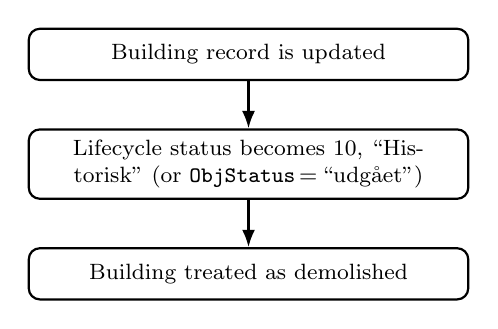
\begin{tikzpicture}[node distance=6mm and 8mm]
\node[ind] (a) {Building record is updated};
\node[ind, below=of a] (b) {Lifecycle status becomes 10, ``Historisk'' (or \texttt{ObjStatus}\,=\,``udg{\aa}et'')};
\node[ind, below=of b] (c) {Building treated as demolished};
\draw[indarrow] (a) -- (b);
\draw[indarrow] (b) -- (c);
\end{tikzpicture}
\caption{Register-exit proxy (indicator~D1): a building leaving the
active stock is treated as demolished. This is the signal behind the
register-exit studies in Table~\ref{tab:lit-indicators}.}
\label{fig:ind-d1}
\end{figure}

\subsubsection*{Event-coded update proxy (Indicator D2)}

This proxy relies entirely on the business-process code attached to a
building's update history (Figure~\ref{fig:ind-d2}). D2 counts a building
whose history ever carried \texttt{ForretningsProcess} 3 (``updated due
to demolition''); the year is the earliest such effect date. D2 is not a
subset of D1: on the current extract, 126{,}362 buildings carry process
3 without ever reaching status 10, so this code is missed by many real
demolitions that are registered through another workflow (undercount).

\begin{figure}[h!]
\centering
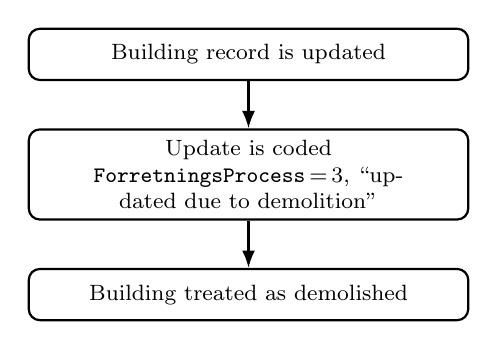
\begin{tikzpicture}[node distance=6mm and 8mm]
\node[ind] (a) {Building record is updated};
\node[ind, below=of a] (b) {Update is coded \texttt{ForretningsProcess}\,=\,3, ``updated due to demolition''};
\node[ind, below=of b] (c) {Building treated as demolished};
\draw[indarrow] (a) -- (b);
\draw[indarrow] (b) -- (c);
\end{tikzpicture}
\caption{Event-coded update proxy (indicator~D2): treats the
demolition-coded record update as the demolition signal.}
\label{fig:ind-d2}
\end{figure}

\subsubsection*{Register exit and demolition process (Indicator D3)}

This proxy fires only where the register exit (D1) coincides with the
demolition-coded update (D2) on the same building
(Figure~\ref{fig:ind-d3}). D3 is the intersection D1 $\cap$ D2, dated by
D1's register-exit year. Because D2 is not a subset of D1, D3 is markedly
smaller than either indicator alone.

\begin{figure}[h!]
\centering
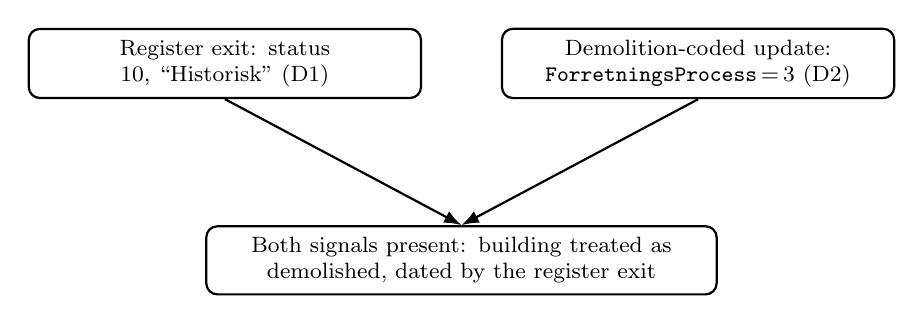
\begin{tikzpicture}[node distance=16mm and 10mm]
\node[ind, text width=4.7cm] (a) {Register exit: status 10, ``Historisk'' (D1)};
\node[ind, text width=4.7cm, right=of a] (b) {Demolition-coded update: \texttt{ForretningsProcess}\,=\,3 (D2)};
\node[ind, text width=6.2cm, below=of $(a.south)!0.5!(b.south)$] (c) {Both signals present: building treated as demolished, dated by the register exit};
\draw[indarrow] (a.south) -- (c.north);
\draw[indarrow] (b.south) -- (c.north);
\end{tikzpicture}
\caption{Intersection proxy (indicator~D3): requires the register exit
(D1) to coincide with the demolition process code (D2).}
\label{fig:ind-d3}
\end{figure}

\subsubsection*{Total demolition case (Indicator D4)}

From here the proxies read the building's linked demolition case rather
than its status history. A case is tied to a building through the
\texttt{stamdataBygning} field on \texttt{Sagsniveau}, which names the
building the case is filed on; D4 keeps only total-demolition cases
(Figure~\ref{fig:ind-d4}). D4 counts a building linked, via
\texttt{Sagsniveau}, to a demolition case of type
\texttt{sagstype}\,=\,32 (``Nedrivning hel,'' total). Partial-demolition
cases (\texttt{sagstype}\,=\,31, ``Nedrivning delvis'') also exist in the
register but qualify no indicator in this study, since a partially
demolished building generally remains standing. The year is the
building's own status-10 date where available, and left undated
otherwise. Roughly 82{,}000 demolition-case rows carry no linkable
building (\texttt{stamdataBygning} null) and are necessarily excluded, an
undercount shared with D6.

\begin{figure}[h!]
\centering
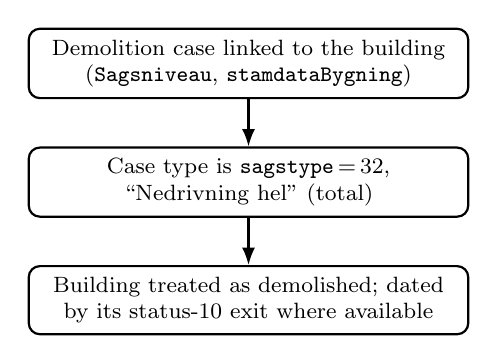
\begin{tikzpicture}[node distance=6mm and 8mm]
\node[ind] (a) {Demolition case linked to the building (\texttt{Sagsniveau}, \texttt{stamdataBygning})};
\node[ind, below=of a] (b) {Case type is \texttt{sagstype}\,=\,32, ``Nedrivning hel'' (total)};
\node[ind, below=of b] (c) {Building treated as demolished; dated by its status-10 exit where available};
\draw[indarrow] (a) -- (b);
\draw[indarrow] (b) -- (c);
\end{tikzpicture}
\caption{Demolition-case proxy, total (indicator~D4): a building linked
to a total-demolition case is treated as demolished, dated by its
register exit.}
\label{fig:ind-d4}
\end{figure}

\subsubsection*{Register exit and total demolition case (Indicator D5)}

This proxy requires the register exit (D1) to coincide with a linked
total-demolition case (D4) on the same building
(Figure~\ref{fig:ind-d5}). D5 is the intersection D1 $\cap$ D4, dated by
D1's register-exit year: a building that both left the active stock and
has a linked total-demolition case.

\begin{figure}[h!]
\centering
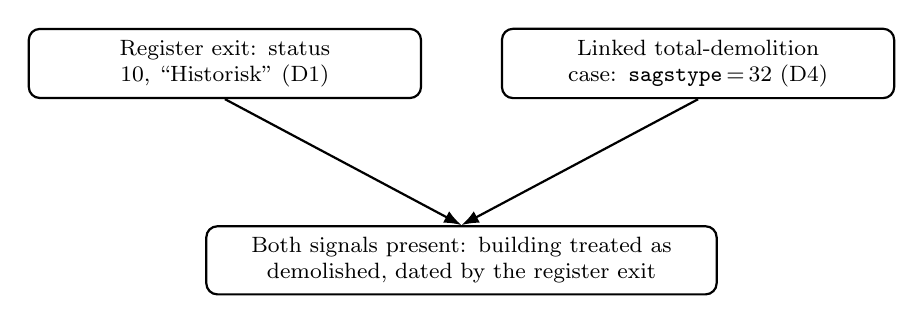
\begin{tikzpicture}[node distance=16mm and 10mm]
\node[ind, text width=4.7cm] (a) {Register exit: status 10, ``Historisk'' (D1)};
\node[ind, text width=4.7cm, right=of a] (b) {Linked total-demolition case: \texttt{sagstype}\,=\,32 (D4)};
\node[ind, text width=6.2cm, below=of $(a.south)!0.5!(b.south)$] (c) {Both signals present: building treated as demolished, dated by the register exit};
\draw[indarrow] (a.south) -- (c.north);
\draw[indarrow] (b.south) -- (c.north);
\end{tikzpicture}
\caption{Intersection proxy (indicator~D5): requires the register exit
(D1) to coincide with a linked total-demolition case (D4).}
\label{fig:ind-d5}
\end{figure}

\subsubsection*{Case-date proxy for felt 295 (Indicator D6)}

D6 dates a linked total-demolition case by its notification date,
standing in for the undistributed completion field felt 295
(Figure~\ref{fig:ind-d6}). D6 counts a building linked to a
total-demolition case (\texttt{sagstype}\,=\,32, as in D4) with a non-null
case notification date (\texttt{sag002 Byggesagsdato}, the approximate
counterpart of the undistributed felt 294 notification field); the year
is that date. Felt 295 itself is not reconstructable from this extract
(Section~\ref{sec:bbr-chain}): the one candidate completion field carried
by the case data (\texttt{sag010 FuldførelseAfByggeri}) is both sparse
and typically dates a co-filed construction case rather than the
demolition, so it is not used. D6 therefore dates demolition
\emph{notification}, not confirmed completion.

\begin{figure}[h!]
\centering
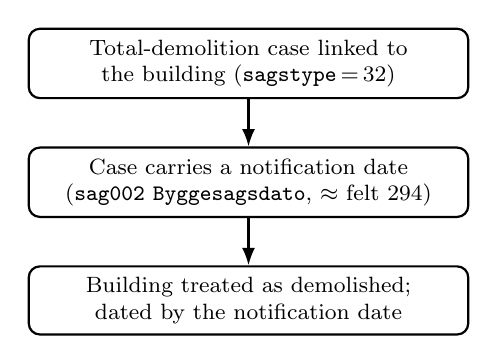
\begin{tikzpicture}[node distance=6mm and 8mm]
\node[ind] (a) {Total-demolition case linked to the building (\texttt{sagstype}\,=\,32)};
\node[ind, below=of a] (b) {Case carries a notification date (\texttt{sag002 Byggesagsdato}, $\approx$ felt 294)};
\node[ind, below=of b] (c) {Building treated as demolished; dated by the notification date};
\draw[indarrow] (a) -- (b);
\draw[indarrow] (b) -- (c);
\end{tikzpicture}
\caption{Case-date proxy (indicator~D6): a linked total-demolition case
is dated by its notification date, an approximation of the undistributed
felt~295 completion signal.}
\label{fig:ind-d6}
\end{figure}

None of D1--D6 is treated as a reference indicator in this study, and
none is scored against another as ground truth; Sections~\ref{sec:comparisons}
and~\ref{sec:results} describe how the six are compared and validated
instead.

\begin{table}[htbp]
\centering
\small
\caption{The demolition-indicator set computed in this study, unfiltered
building counts windowed to 2000--2025 (denominator: 6{,}250{,}075
buildings in the extract).}
\label{tab:d-indicators}
\begin{tabular}{@{}lp{7.4cm}r@{}}
\toprule
ID & Signal & Buildings \\
\midrule
D1 & status = 10 & 436{,}194 \\
D2 & forretningsproces = 3 & 225{,}706 \\
D3 & D1 $\cap$ D2 & 99{,}664 \\
D4 & sagstype = 32 (total) & 237{,}012 \\
D5 & D1 $\cap$ D4 & 200{,}634 \\
D6 & sagstype = 32 with notification date & 231{,}962 \\
\bottomrule
\end{tabular}
\end{table}

\subsection{Demolition indicators in prior register-based studies}\label{sec:lit-indicators}

Table~\ref{tab:lit-indicators} lists the approach and key filters used
by published Danish studies that estimate building demolition from BBR or
a BBR-derived extract, and, in its second column, the indicator in the
set above (Section~\ref{sec:ind-set}) that rests on the same register
signal. The register-exit and event-coded studies map directly onto D1
and D2. Two further approaches used in the literature have no direct
counterpart in the D1--D6 set, because both reach outside the register
signals this study computes: studies working from a pre-made, opaque
demolition extract, whose filtering recipe is not
published;\footnote{The recipe is unpublished, but the underlying signal is
recoverable. For the one such extract we hold --- the KMD/Andersen
extract~\cite{andersen2022adaptation} --- every case is a total demolition
(\texttt{sagstype = 32}), and the case-based indicator reproduces its
membership to $\sim$99\,\% window-matched (Section~\ref{sec:kmd}). So it
corresponds empirically to the case family D4--D6, even though the authors
state no register field that identifies it.} and change-detection studies,
which infer demolition from a teardown-and-rebuild sequence rather than
from a demolition signal on the building itself.

Two entries in Table~\ref{tab:lit-indicators} fall outside the proxy
scheme entirely. SBi's evaluation of village-renewal demolition
subsidies~\cite{jensen2019landsbyfornyelse} additionally draws on
BOSSINF, the administrative register of grant-funded demolitions: this
is genuine ground truth rather than a proxy, but limited to subsidised
cases in 54 eligible municipalities. Aagaard et
al.~\cite{aagaard2013levetider} do not detect individual demolitions at
all; they assume an aggregate demolition rate ($\approx$0.3\,\%/yr)
derived from construction-cost statistics, which underlies the standard
Danish service-life tables and is the baseline that later extract-based
studies benchmark against.

\begin{table}[h!]
\centering
\small
\renewcommand{\arraystretch}{1.2}
\setlength{\tabcolsep}{5pt}
\newcolumntype{L}[1]{>{\raggedright\arraybackslash}p{#1}}
\caption{Demolition indicators (proxies) and filters used in prior
published Danish register-based studies, and the corresponding indicator
in this study's set (Section~\ref{sec:ind-set}).}
\label{tab:lit-indicators}
\begin{tabular}{@{}L{0.25\linewidth}L{0.31\linewidth}L{0.34\linewidth}@{}}
\toprule
Study & Approach (corresponding indicator) & Key filters \\
\midrule
Aagaard et al.\ (2013)~\cite{aagaard2013levetider} &
  Not a detection method (n/a) &
  n/a \\
\addlinespace[2pt]\cmidrule(l{0pt}r{0pt}){1-3}\addlinespace[2pt]
{\O}stergaard et al.\ (2018)~\cite{ostergaard2018temporal} &
  Opaque extract (no direct D-indicator) &
  Missing/duplicate records dropped; lifespan $<5$\,yr dropped; built
  before 1800 dropped \\
\addlinespace[2pt]\cmidrule(l{0pt}r{0pt}){1-3}\addlinespace[2pt]
SBi (2019:01)~\cite{jensen2019landsbyfornyelse} &
  Register-exit (D1); plus BOSSINF ground truth &
  Residential codes only; 54 eligible municipalities \\
\addlinespace[2pt]\cmidrule(l{0pt}r{0pt}){1-3}\addlinespace[2pt]
Andersen \& Negendahl (2022)~\cite{andersen2022adaptation} &
  Opaque extract (no direct D-indicator) &
  Pre-2011 records discarded \\
\addlinespace[2pt]\cmidrule(l{0pt}r{0pt}){1-3}\addlinespace[2pt]
BUILD (2022:36)~\cite{jensen2022enfamiliehuse} &
  Change detection, BBR flag (outside D1--D6) &
  Code 120 only; same matrikel; rebuild after 2010 \\
\addlinespace[2pt]\cmidrule(l{0pt}r{0pt}){1-3}\addlinespace[2pt]
Andersen \& Negendahl (2023)~\cite{andersen2023lifespan} &
  Opaque extract (no direct D-indicator) &
  Missing date/area/use dropped; pre-2010 dropped; construction year
  ``1000'' (auto-generated) dropped \\
\addlinespace[2pt]\cmidrule(l{0pt}r{0pt}){1-3}\addlinespace[2pt]
Boligøkonomisk Videncenter (2023)~\cite{blv2023karakteristika} &
  Change detection, transaction (outside D1--D6) &
  Arms-length sales only; plot 500--2{,}000\,m$^2$; price
  15--15{,}000\,kr/m$^2$; matrikel age $\geq$20\,yr \\
\addlinespace[2pt]\cmidrule(l{0pt}r{0pt}){1-3}\addlinespace[2pt]
BUILD (2025)~\cite{jensen2025nedrivning} &
  Register-exit (D1) &
  Buildings built before 1999 only \\
\addlinespace[2pt]\cmidrule(l{0pt}r{0pt}){1-3}\addlinespace[2pt]
Droob et al.\ (2026)~\cite{droob2026servicelife} &
  Event-coded update (D2) &
  Outbuildings removed \\
\bottomrule
\end{tabular}
\end{table}

%% =========================================================================
\section{Methods}\label{sec:methods}

The demolition indicators D1--D6 (Section~\ref{sec:indicators}) are
applied to the cleaned extract of Section~\ref{sec:data}. This section
describes the remaining analysis choices: the treatment of discontinued
use codes, the floor-area measure, the quantities computed
for each indicator, and the planned comparisons.

\subsection{Treatment of discontinued use codes}\label{sec:discontinued-method}

A fixed set of retired, round-number building-use codes (agricultural
and industrial categories no longer issued) is associated with an
ambiguous status-10 signal: earlier work found that a status-10 event on
these codes sometimes reflects administrative re-registration rather
than physical demolition. Rather than building this into a separate
indicator, it is implemented as an orthogonal, on/off exclusion axis
applicable to any of D1--D6 (Section~\ref{sec:indicators}); applying it
to D1 reproduces the earlier inclusive/filtered contrast directly (D1:
436{,}194 buildings; D1 with the exclusion applied: 302{,}261). Whether
excluding these codes should be treated
as a correction is, on the current extract, an open empirical question
rather than an assumption: the exclusion strips approximately 34\,\% of
every indicator's buildings uniformly, consistent with a base rate
across the stock rather than concentrated artifacts, and among the
status-10 buildings it would remove, 50.7\,\% also carry a formal
demolition case, against a 44.2\,\% case-rate among the buildings it
would keep --- so on this extract the exclusion also removes buildings
with independent demolition evidence. Crossing every indicator with the
axis on and off gives the full $7\times2$ comparison grid used in the
ablation (Section~\ref{sec:comparisons}); whether the exclusion improves
or worsens agreement with ground truth is intended to be settled against
BOSSINF (Section~\ref{sec:comparisons}), not assumed.

\subsection{Floor-area measure}\label{sec:areas}

The primary area outcome is total building area,
\texttt{byg038SamletBygningsareal}. This is the area concept used for the
main demolished-square-metre totals and, where a stock denominator is
available, for demolition rates by area. We use a single primary area
field so that the ablation isolates the demolition indicator: the
building set changes from D1 to D6, while the area definition is held
fixed.

This choice is also a comparability decision. \texttt{byg038} is BBR's
registered total floor area and is the closest single field to the area
concept used in service-life, building-stock, and material-flow
applications. Its limitation is coverage, not interpretation:
Section~\ref{sec:missingness} shows that \texttt{byg038} is missing for a
large and non-random part of the stock, especially small outbuildings.
Therefore a building with missing total area remains in the demolition
count, but contributes no square metres to the area total; the number and
share of buildings with non-missing total area are reported alongside the
area estimates. Negative \texttt{byg038} values are excluded after
candidate-event detection using the same rule for every indicator. Zero
values are retained as recorded zero-area observations and reported in
the coverage diagnostics rather than being treated as positive demolished
area.

Other BBR area fields are retained as diagnostics and sensitivity checks,
but not as co-equal headline outcomes. The footprint
\texttt{byg041BebyggetAreal} is nearly complete for historical buildings,
but it measures ground coverage rather than floor area and is therefore
not a substitute for \texttt{byg038}. The sum of residential and
commercial area (\texttt{byg039}+\texttt{byg040}) is useful for comparison
with BUILD's published analysis~\cite{jensen2025nedrivning}, but it is a
different constructed area definition. These alternatives are reported as
robustness or appendix material rather than used to define the main
indicator comparison. A hybrid or imputed area measure---for example,
filling missing total area from footprint and storeys---could be useful
for estimating a more complete physical area flow, but it would introduce
an additional modelling assumption and is therefore left outside the main
indicator-sensitivity analysis.

\subsection{Computed quantities}\label{sec:metrics}

For each indicator, the following are computed by year: the number of
demolitions; the demolished total area; the average and median demolished
area per building; the coverage of \texttt{byg038}; and the demolition
rate relative to the building stock where a valid denominator can be
constructed. The same filters and aggregation logic are used for all
indicators. Results are computed nationally, and by building-use group,
region, and construction period where counts allow. For comparability of
disaggregated results, use codes are grouped according to the 22-group
mapping used by BUILD~\cite{jensen2025nedrivning}.
\groupdecision{exact headline metric (annual demolished m$^2$; share of
stock m$^2$ per year; count-based rates) --- open question \#1 in the
project notes.}

As defined in Section~\ref{sec:data}, annual series are produced over
the full reporting window (2000--2025), while headline averages,
windowed overlap, and rate comparisons use the main comparison window
(2018--2025). The KMD comparison uses its own external-anchor window
(2011--2019).

\subsection{Planned comparisons}\label{sec:comparisons}

%% From the analysis plan (docs/plan.md, Analyses 2, 7, 8): indicator
%% overlap; BUILD reproduction; overlap with the independent extract.
Three comparisons are planned alongside the scenario grid.
\emph{Indicator agreement:} which buildings (and how much area) each
indicator identifies, pairwise and jointly.
\emph{BUILD:} a reproduction of BUILD's analysis setup---buildings
constructed before 1999, retired 2012--2023, area as residential plus
commercial floor area---against their published totals
(Section~\ref{sec:build-comparison})~\cite{jensen2025nedrivning}.
\emph{Independent demolition data:} overlap with an independently
compiled national extract of reported demolition cases (2000--2020)
previously used in published service-life
research~\cite{andersen2022adaptation, andersen2023lifespan}, treated as
a comparison source rather than ground truth, and with the register of
grant-funded demolitions used in the evaluation of the village-renewal
demolition subsidies~\cite{jensen2019landsbyfornyelse}.
\groupdecision{final scope of the validation comparisons --- which of
these are in the paper versus supplementary material.}

%% =========================================================================
\section{Results}\label{sec:results}

\draftnote{Writing guide (2026-07-11, verified against a fresh
\texttt{ablation.py} run; updated 2026-07-12 after the \texttt{rates.py}
run): each subsection below carries a \texttt{\%\%} comment block with the
concrete numbers to write from and the narrative beats, in the order we
agreed. Sections~\ref{sec:overlap}--\ref{sec:kmd} are fully backed by
\texttt{results/} and ready to draft now; \ref{sec:missingness} is
optional-now (data-quality preamble); \ref{sec:rate-vs-stock}
and~\ref{sec:build-comparison} are now backed by
\texttt{results/rates\_*.csv} (2026-07-12) and drafted below. Draft order:
overlap $\to$ annual $\to$ discontinued $\to$ area $\to$ KMD $\to$ rates.}

%% ---- SOURCE FILES (real names, verified) --------------------------------
%%   results/ablation_summary.csv  — one row / 12 variants: counts + 3 area
%%                                   defs (footprint/total/etage) w/ median
%%                                   + coverage%%
%%   results/annual.csv            — variant x year: count + m2 per area def
%%   results/by_region.csv         — variant x region: count + etage m2
%%   results/overlap.csv           — pairwise intersection + Jaccard (D1-D6)
%%   results/overlap_2018_2025.csv — same, restricted to dated 2018-2025
%%   results/kmd_comparison.csv    — each proxy vs KMD extract (raw + window)
%%   results/cleaning_report.csv   — cleaned values per rule, per indicator
%%   results/data_quality_*.csv    — from src/data_quality.py (NOT ablation)
%%   results/rates_summary.csv     — variant x window: mean rate + coverage
%%                                   + m2/yr, both pairings (src/rates.py)
%%   results/rates_spread.csv      — window x pairing: min/max variant + fold
%%   results/rates_annual.csv      — variant x year 2011-2025: rate series
%%   results/stock_national.csv    — parsed BYGB34 national stock per year
%%   results/figures/*.png|pdf     — annual_counts, annual_area_total,
%%                                   overlap_heatmap, overlap_heatmap_2018_2025
%%                                   (rate_vs_stock came from src/rates.py, which is
%%                                   not in this checkout — regenerate before reuse)

\subsection{Indicator overlap}\label{sec:overlap}
%% STATUS: READY. Sources: overlap.csv + counts from ablation_summary.csv.
%%   Figure: results/figures/overlap_heatmap.png. This is the SPINE of the
%%   paper — the proxies genuinely disagree; everything downstream is the
%%   consequence. Lead with it.
%% NARRATIVE BEATS:
%%  1. COUNT SPREAD. The six indicators, same window (2000-2025), same
%%     extract, disagree by a factor of ~4.4x on how many buildings were
%%     demolished:
%%        D1 status=10                 436,194   (most inclusive)
%%        D4 sagstype=32               237,012
%%        D6 total case, sag002 dated  231,962
%%        D2 forretningsproces=3       225,706
%%        D5 status10 & sagstype=32    200,634
%%        D3 status10 & proces=3        99,664   (least inclusive)
%%     Even the two "canonical" single signals — register-exit (D1) vs
%%     event-code (D2) — differ nearly 2x.
%%  2. THE TWO CANONICAL PROXIES BARELY AGREE. D1 vs D2 Jaccard = 0.177;
%%     their intersection is only 99,664 buildings (= all of D3). So
%%     status=10 and forretningsproces=3 identify largely DIFFERENT
%%     buildings. D2 is NOT a subset of D1: 126k buildings are process-3
%%     but never status-10 (report from docs; = 225,706 - 99,664).
%%  3. THE CASE-BASED FAMILY IS TIGHT. D4/D5/D6 cluster at Jaccard
%%     0.85-0.92: D4-D6 0.918, D5-D6 0.853, D4-D5 0.847. So "which
%%     demolition-case variant" barely matters; "case-based vs
%%     register-exit vs event-code" matters enormously.
%%  4. CROSS-FAMILY LOW: D1 vs case-family ~0.42-0.46 (D1-D5 0.460,
%%     D1-D4 0.425, D1-D6 0.424); D2 vs everything 0.18-0.44.
%%  INTERPRETATION: the choice of proxy is not cosmetic. Disagreement
%%  between indicators IS the result, not noise to resolve against a
%%  reference (there is no gold label — see indicators section).
The six indicators pick out very different sets of demolished buildings
(Table~\ref{tab:overlap-size}). The count ranges from 99{,}664 buildings
(D3) to 436{,}194 (D1) --- a 4.4-fold difference --- and their total floor
area (\texttt{byg038}) ranges from 13.5 to 44.7~million~m\textsuperscript{2}.
The area figures depend not only on which buildings an indicator selects,
but also on how many of them have a recorded area, and that share differs
by indicator (Section~\ref{sec:area-sensitivity}).

\begin{table}[htbp]
\centering
\caption{Number of demolished buildings and their total floor area
(\texttt{byg038}) under each indicator, 2000--2025.}
\label{tab:overlap-size}
\begin{tabular}{llrr}
\toprule
Indicator & Signal & Buildings & Floor area (M\,m\textsuperscript{2}) \\
\midrule
D1 & \texttt{status = 10}                    & 436{,}194 & 44.7 \\
D2 & \texttt{forretningsproces = 3}          & 225{,}706 & 16.1 \\
D3 & D1 $\cap$ D2                            &  99{,}664 & 13.5 \\
D4 & \texttt{sagstype = 32}                  & 237{,}012 & 34.5 \\
D5 & D1 $\cap$ D4                            & 200{,}634 & 26.6 \\
D6 & \texttt{sagstype = 32}, notification date & 231{,}962 & 33.7 \\
\bottomrule
\end{tabular}
\end{table}

Figure~\ref{fig:overlap-heatmap} shows how much the sets overlap, measured
by the Jaccard index (the buildings two indicators share, divided by the
number in either one). D1 (\texttt{status = 10}) and D2
(\texttt{forretningsproces = 3}) overlap by only 0.18: they share 99{,}664
buildings, which means 126{,}042 of D2's buildings never reach
\texttt{status = 10}. The three demolition-case indicators D4, D5 and D6
overlap each other much more, at 0.85--0.92, while each overlaps D1 at
0.42--0.46 and D2 at 0.28--0.30.

\begin{figure}[htbp]
\centering
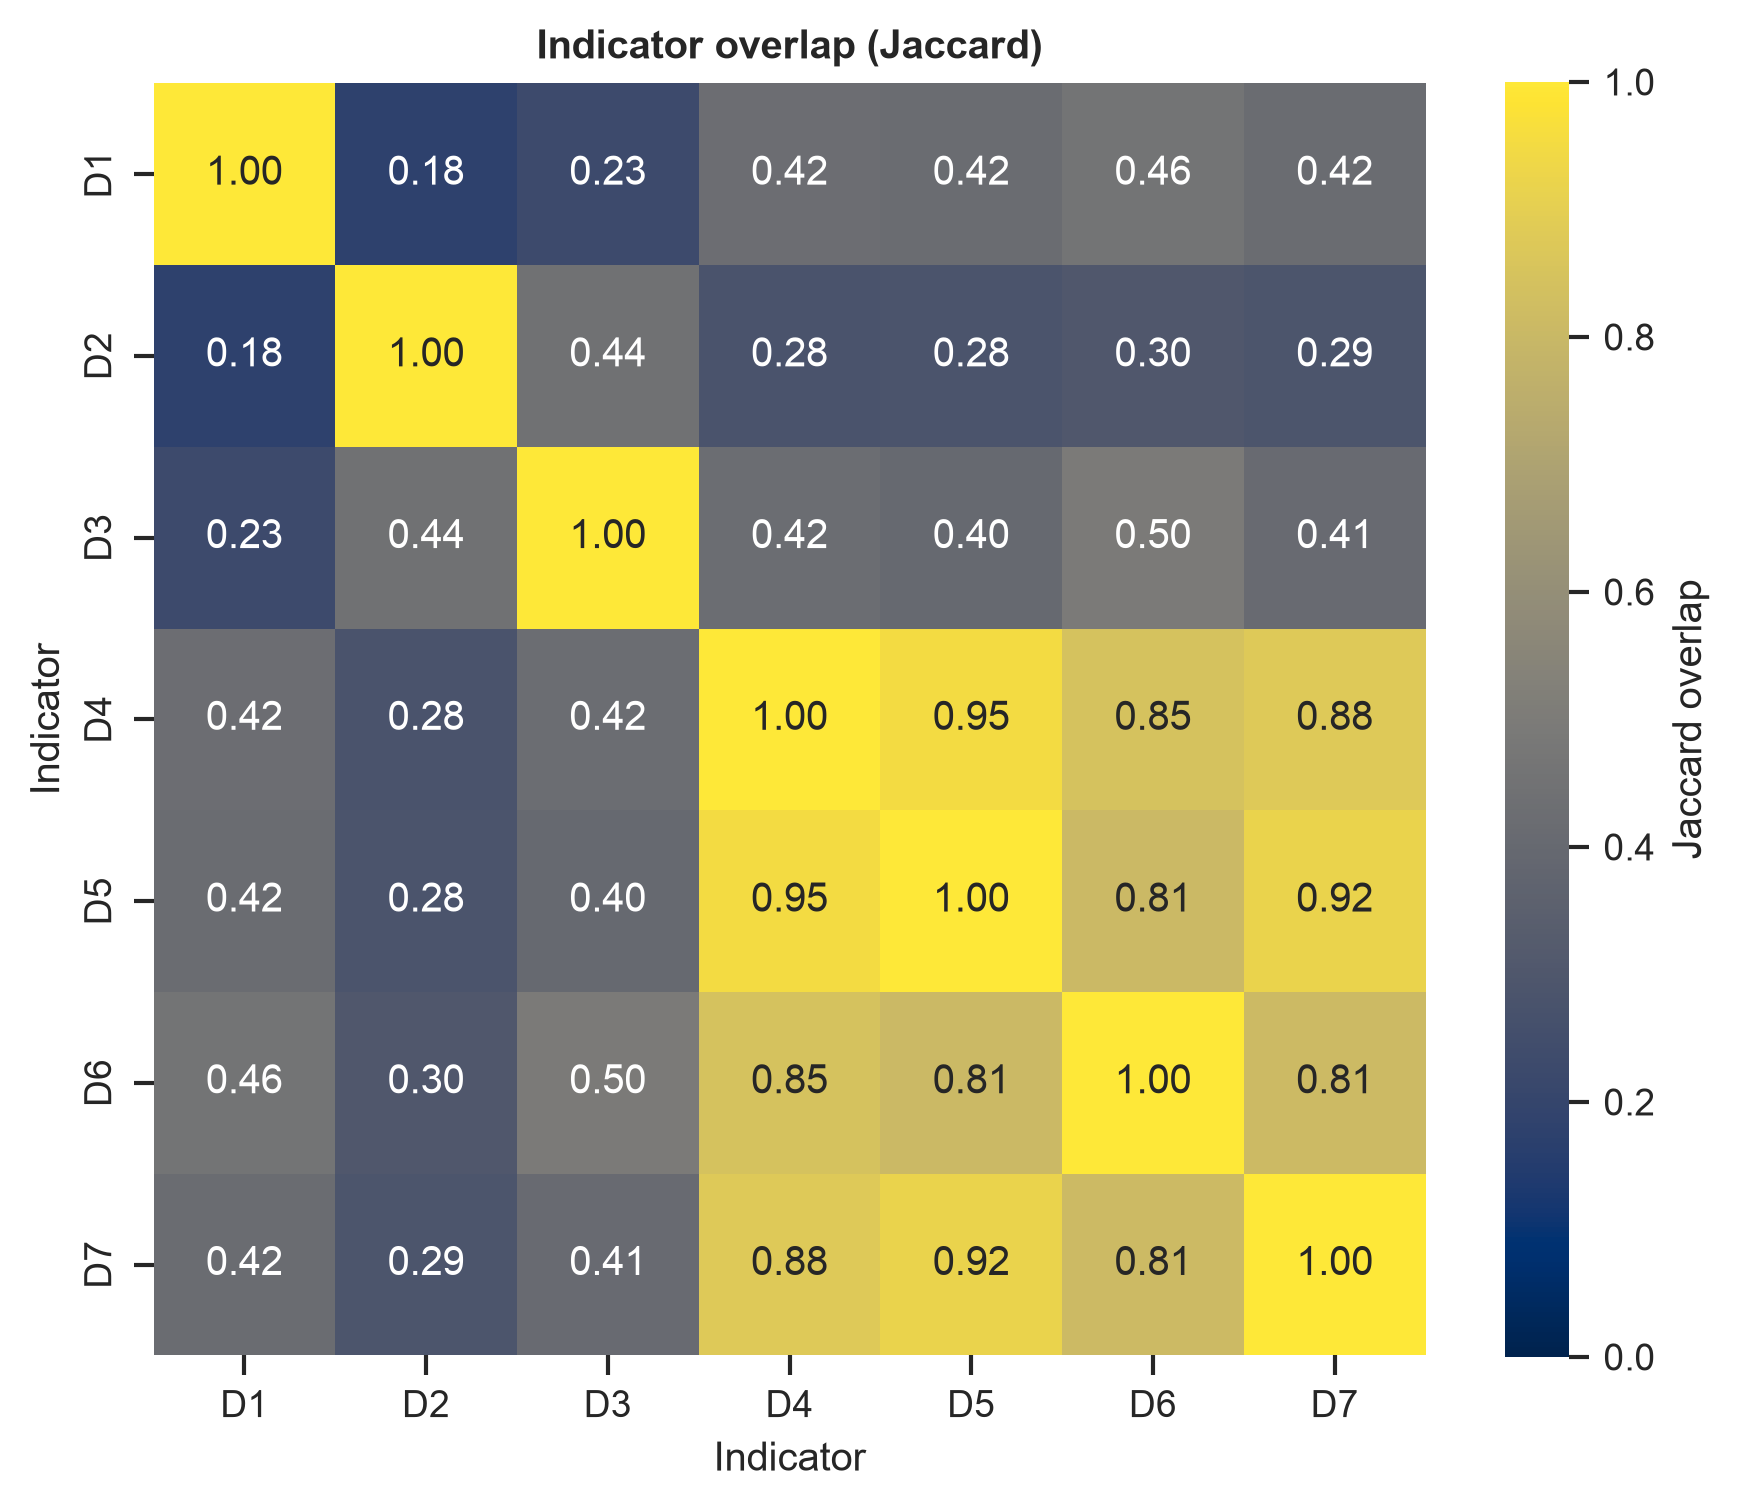
\includegraphics[width=0.7\textwidth]{media/overlap_heatmap.png}
\caption{How much the six indicators' sets of demolished buildings
overlap, measured by the Jaccard index (2000--2025).}
\label{fig:overlap-heatmap}
\end{figure}

Restricting the comparison to dated memberships in the stable 2018--2025
window changes the pattern but not the main conclusion
(Figure~\ref{fig:overlap-heatmap-2018}). The inclusive register-exit
indicator D1 remains the broad outlier: its overlap with D2 is 0.38 and
with the total-demolition-case indicators D4/D5 is 0.42. By contrast,
D2, D3, D4 and D5 form a much tighter recent-period cluster, with
Jaccard values of 0.87--1.00. This shows that part of the weak full-window
agreement is a period and dating issue rather than only a membership
issue. In this dated-window table D4 and D5 are identical because D4 is
dated by the building's status-10 year; D4 case-only members without a
status-10 year are therefore excluded from the windowed comparison. The
notification-dated case indicator D6 overlaps the same cluster
less strongly, at 0.65--0.67, because it assigns the year from the case
date rather than from the status-10 register exit.

\begin{figure}[htbp]
\centering
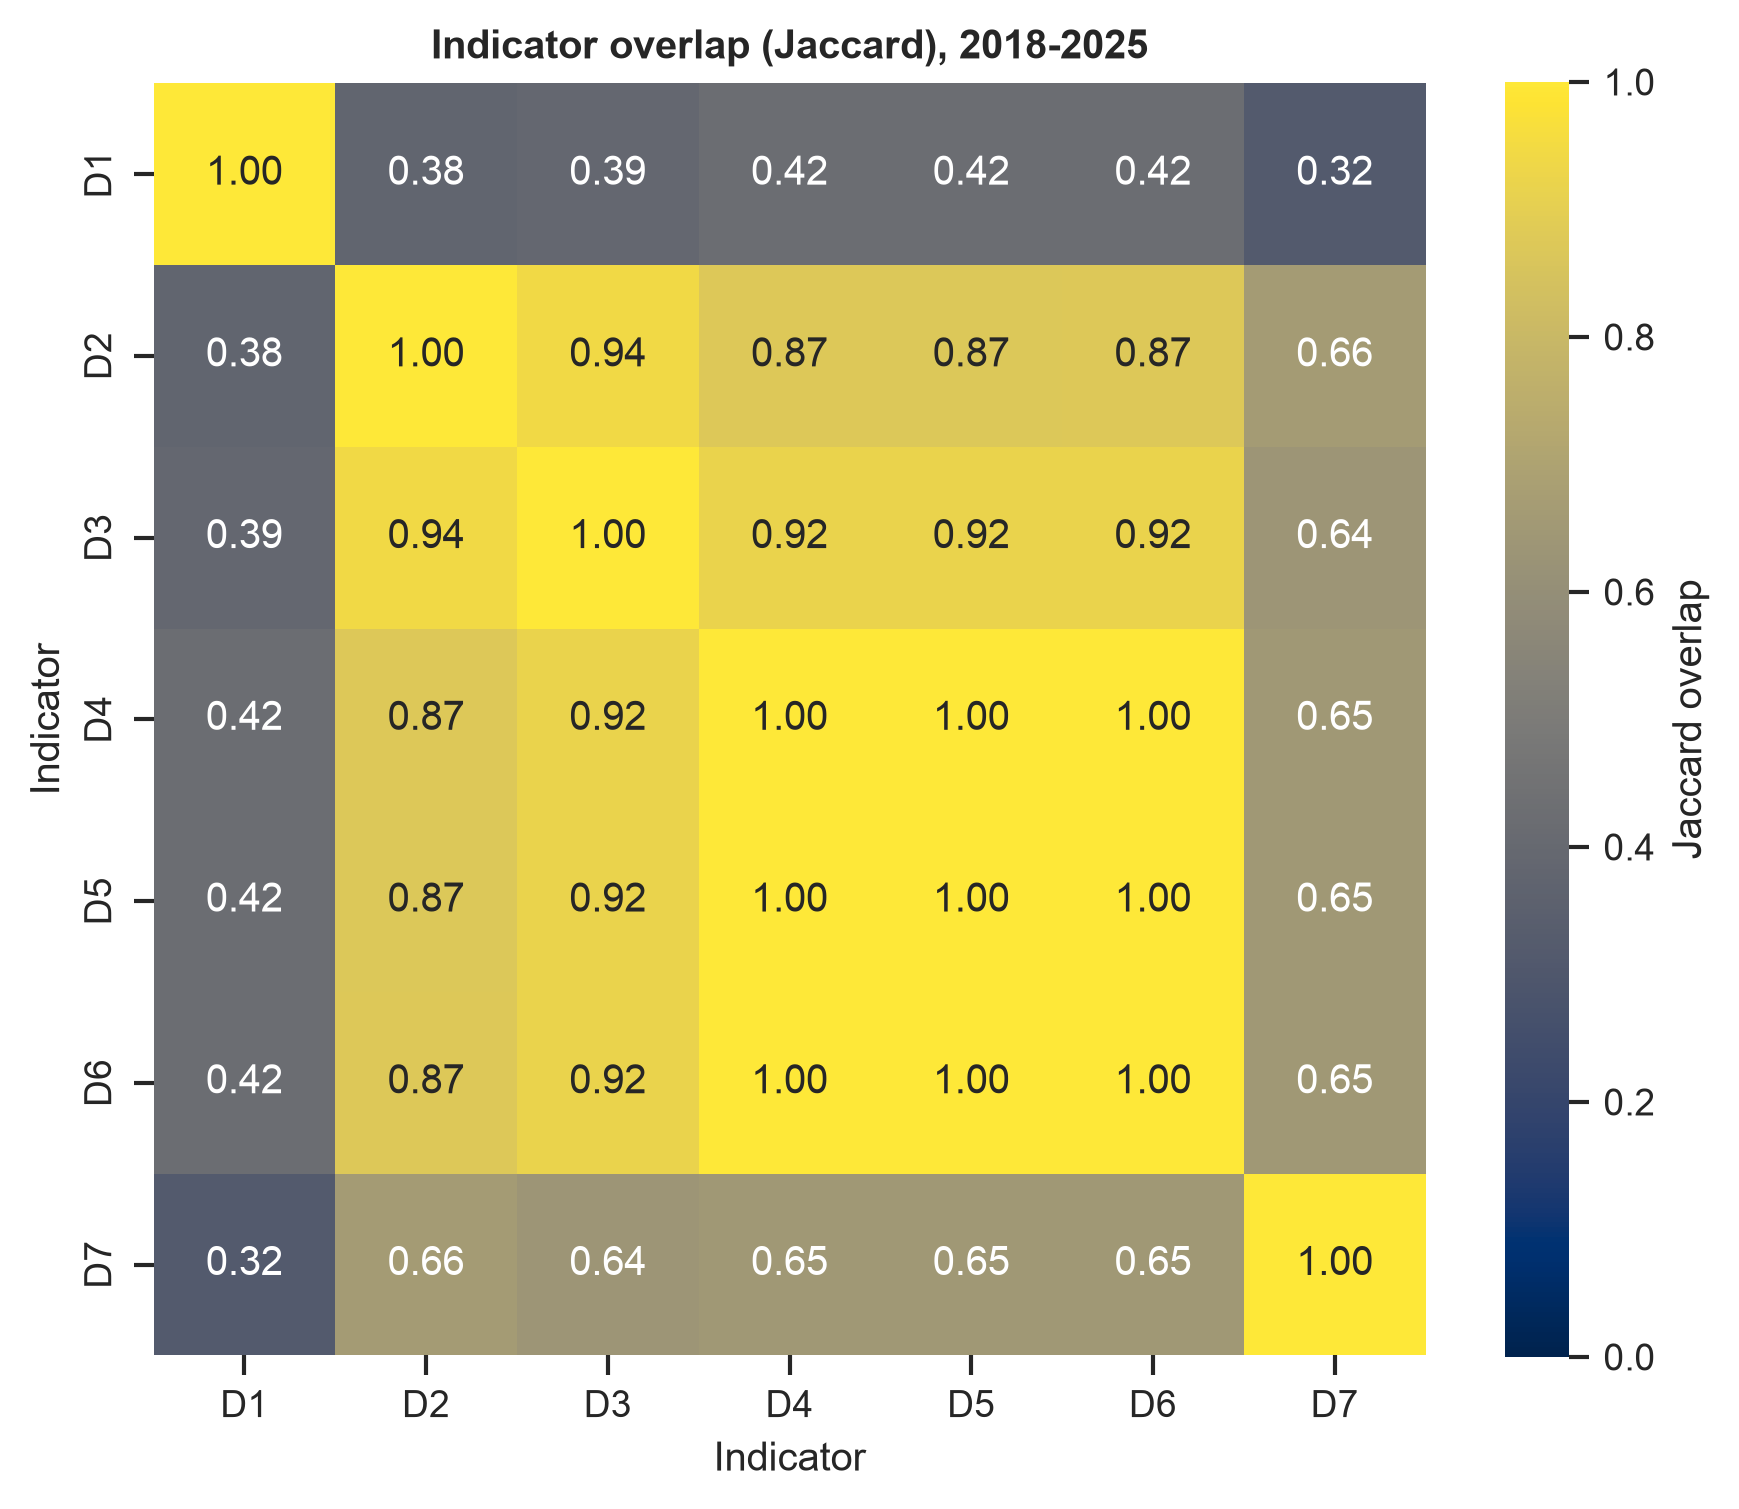
\includegraphics[width=0.7\textwidth]{media/overlap_heatmap_2018_2025.png}
\caption{Indicator overlap restricted to dated memberships in the
2018--2025 comparison window. The higher agreement among D2--D5 shows the
recent-period convergence of the process and case-based signals; D6 is
partly separated by its notification-date clock.}
\label{fig:overlap-heatmap-2018}
\end{figure}

\subsection{Annual demolition estimates by indicator}\label{sec:rates}
%% STATUS: READY. Sources: annual.csv (+ ablation_summary totals).
%%   Figures: annual_counts.png, annual_area_total.png. This is the
%%   ablation's payload: same computation, swap indicator, watch the
%%   national series move.
%% NARRATIVE BEATS:
%%  1. THE SPREAD PERSISTS EVERY YEAR. For a representative recent complete
%%     year (2022): D1=32,874 buildings, D4=16,026, D6=13,033.
%%     Report the annual count envelope across indicators, not one line.
%%  2. AREA/YR ENVELOPE (byg038 total m2): 2018-2025 means run 2.84M m2/yr
%%     for D1, 1.72M for D4/D5, 2.14M for D6. Give the range; this is
%%     what feeds any stock-turnover / LCA reference figure.
%%  3. TWO ARTIFACTS TO CAVEAT (do NOT hide these):
%%     (a) YEAR-2000 PILE-UP. Backdated virkningFra below the 2000 clamp
%%         all lands on 2000: D1=24,550 in 2000 vs ~300-1,600/yr for
%%         2001-2010; D4=14,056 in 2000. D6 (notification-dated) does NOT
%%         pile up (25 in 2000) — good illustration that the artifact is a
%%         register-exit dating effect, not real activity. => the
%%         comparable window is ~2011/2012-2025, not 2000.
%%     (b) 2011 STEP-UP. All register-exit series jump at 2011 (BBR
%%         registration reforms) — pre-2011 is not comparable.
%%  4. UNDATED CASE MEMBERS. D4 has members with no status-10 year, so
%%     they sit in the totals but not the time series: D4 n_dated=200,634
%%     of 237,012 (D4's dated subset = D5). State this so the annual D4
%%     line reads lower than its total.
%%  WINDOW DECISION: Section~\ref{sec:data} defines 2000--2025 as the full
%%  reporting window and 2018--2025 as the main comparison window.
Figure~\ref{fig:annual} shows the demolitions per year under each
indicator: counts in panel~(a) and demolished total floor area in
panel~(b), across the full 2000--2025 window. The differences between
indicators seen in Section~\ref{sec:overlap} continue year by year: the
curves have the same shape but stay separated by roughly the same multiple
throughout. We compare numbers only over the complete years 2018--2025
(Section~\ref{sec:methods}), where all indicators are reliable;
Table~\ref{tab:annual-mean} gives each indicator's average over those eight
years.

\begin{table}[htbp]
\centering
\caption{Average demolitions per year and demolished floor area per year
(\texttt{byg038}) under each indicator, 2018--2025.}
\label{tab:annual-mean}
\begin{tabular}{llrr}
\toprule
Indicator & Signal & Buildings/yr & Floor area (M\,m\textsuperscript{2}/yr) \\
\midrule
D1 & \texttt{status = 10}              & 30{,}369 & 2.84 \\
D2 & \texttt{forretningsproces = 3}    & 12{,}458 & 1.89 \\
D3 & D1 $\cap$ D2                      & 11{,}748 & 1.60 \\
D4 & \texttt{sagstype = 32}            & 12{,}708 & 1.72 \\
D5 & D1 $\cap$ D4                      & 12{,}708 & 1.72 \\
D6 & \texttt{sagstype = 32}, notification date & 14{,}433 & 2.14 \\
\bottomrule
\end{tabular}
\end{table}

Over 2018--2025 the yearly count runs from about 11{,}700 (D3) to
30{,}400 (D1). In every single year the highest indicator is 2.2 to 3.1
times the lowest. D1 sits at roughly twice the demolition-case indicators,
which group near 12{,}700/yr (D4 and D5); D6 is a little higher, at
about 14{,}400/yr. The gap in demolished area is smaller: yearly totals
average 1.6 to 2.8~million~m\textsuperscript{2}. D1's area is only about
1.6 times the case indicators, less than its 2.4-times lead in counts --- so
the extra buildings D1 picks up tend to be smaller and less often have a
recorded area (Sections~\ref{sec:overlap} and~\ref{sec:area-sensitivity}).

The years before 2011 are not comparable and are shown only for
completeness, because of two dating effects. First, dates that were
backdated to before the start of the window all pile up on the year 2000:
D1 shows 24{,}550 buildings in 2000 against 600--1{,}150 per year in the
mid-2000s, and D4 shows 14{,}056. D6, which is dated from the demolition
notice, shows no such spike (25 in 2000). Second, the register-exit and
case indicators jump upward in 2011, after a BBR registration reform (D1:
1{,}150 in 2010, 12{,}670 in 2011, 22{,}546 in 2012). D6 instead already
has large counts in 2009--2010, when the others are close to zero --- these
are the same demolitions, but dated from the notice rather than from the
register exit. So the indicators disagree not only on which buildings count
as demolished, but also on \emph{when} the demolition happened.

Finally, the demolition-case indicator D4 includes buildings that
never reached \texttt{status = 10} and so have no year attached: 200{,}634
of D4's 237{,}012 buildings have a date. The undated ones count toward the
totals in Table~\ref{tab:overlap-size} but not toward the yearly series, so
D4's yearly line sits below its total and matches D5.

\begin{figure}[htbp]
\centering
\begin{subfigure}[t]{0.49\textwidth}
  \centering
  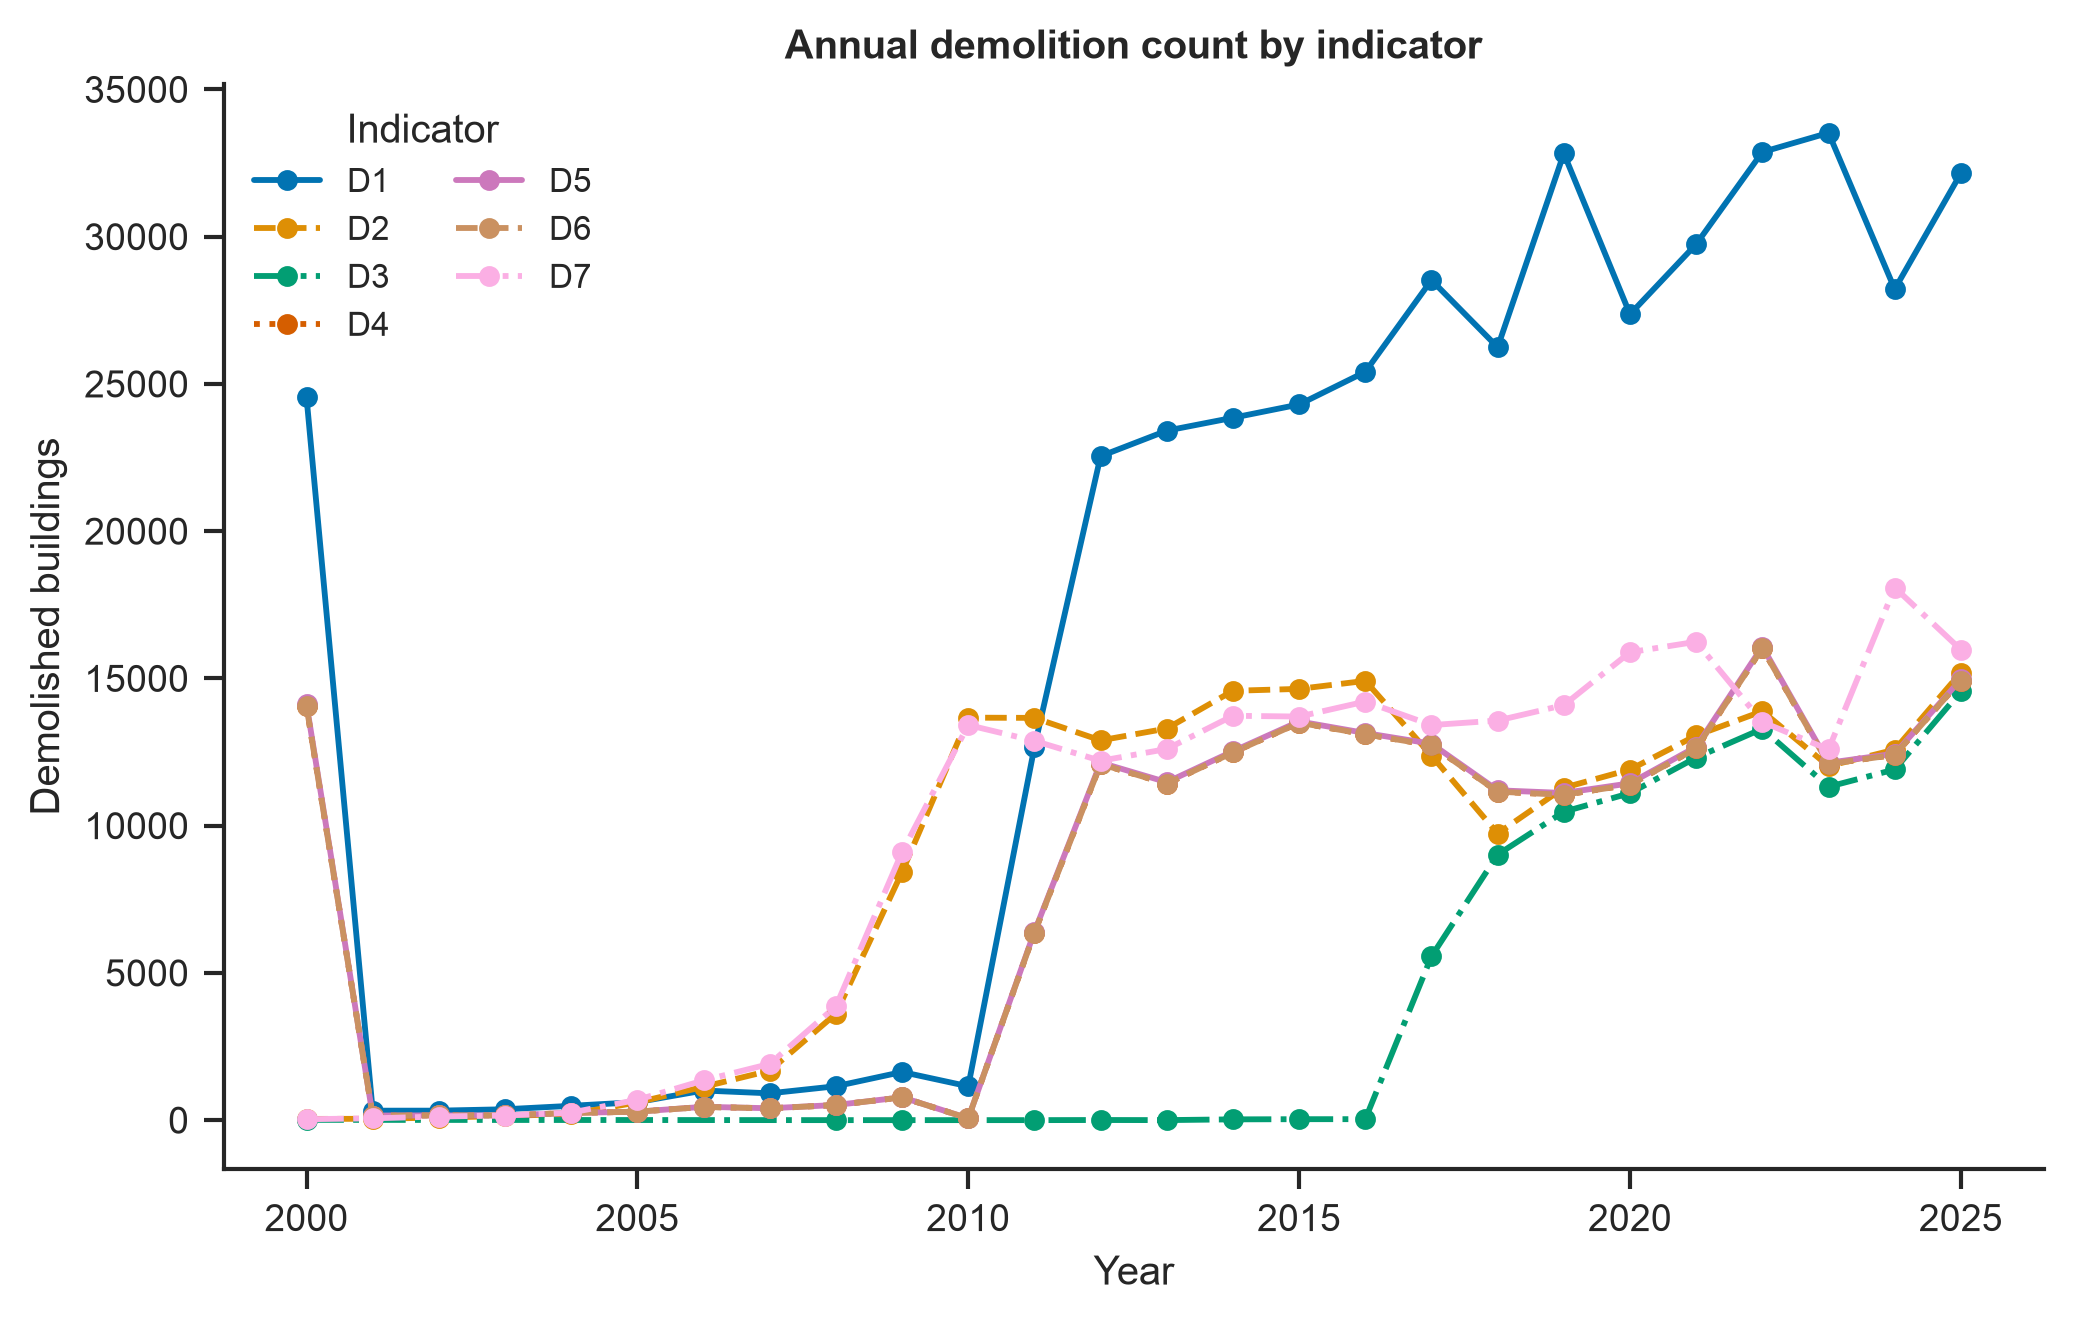
\includegraphics[width=\textwidth]{media/annual_counts.png}
  \caption{Demolition counts.}
  \label{fig:annual-counts}
\end{subfigure}
\hfill
\begin{subfigure}[t]{0.49\textwidth}
  \centering
  
\includegraphics[width=\textwidth]{media/annual_area_total.png}
  \caption{Demolished floor area.}
  \label{fig:annual-area}
\end{subfigure}
\caption{Annual demolition series per indicator, 2000--2025:
(a)~building counts and (b)~demolished floor area.}
\label{fig:annual}
\end{figure}

\subsection{Discontinued-code analysis}\label{sec:discontinued}
%% STATUS: READY. Sources: the -exdisc variants in ablation_summary.csv.
%%   THE STRONGEST SELF-CONTAINED FINDING. Headline: the discontinued-code
%%   exclusion is an AREA story, not a count story.
%% NARRATIVE BEATS:
%%  1. COUNTS MOVE MODESTLY, AREA COLLAPSES. Excluding discontinued round-
%%     number use-codes from D1:
%%        count   436,194 -> 302,261   (-31%)
%%        etage   47.5M  -> 9.9M m2     (-79%)
%%        total   44.7M  -> 9.1M m2     (-80%)
%%        footprint 50.1M -> 15.5M m2   (-69%)
%%     A one-third count cut wipes out four-fifths of the demolished area.
%%  2. UNIFORM STRIP = BASE RATE, NOT ARTIFACT. The exclusion removes
%%     ~31-35% of EVERY indicator's buildings (D4 237,012->155,299 = -34%).
%%     That uniformity says ~a third of the stock carries these old
%%     agricultural/industrial codes — a base rate, not concentrated
%%     re-registration artifacts (contrast the thesis's >90%-fake premise).
%%  3. WHAT IT REMOVES IS THE BIG BUILDINGS. The excluded round-number
%%     codes are large agricultural structures carrying disproportionate
%%     m2 — matches BUILD's finding that landbrug dominates demolished
%%     area. (Median etage m2 also drops, D1 117 -> 100.)
%%  4. IT ALSO REMOVES GENUINE DEMOLITIONS. Of the status-10 buildings the
%%     exclusion drops, 50.7% ALSO carry a formal demolition case (vs 44.2%
%%     among those it keeps) — so it over-corrects. (methods sec covers
%%     this; keep the empirical claim here.)
%%  INTERPRETATION: any headline demolished-m2 figure is hostage to this
%%  single filter choice — a decision that barely moves the building count.
%%  Whether the exclusion is a "correction" is unresolved (settle vs
%%  BOSSINF, future work), so we report inclusive AND excluded side by side.
\pending{inclusive vs -exdisc counts and area for each indicator; the
count-vs-area asymmetry (-31\% count / -79\% area on D1)}

\subsection{Total-floor-area coverage and robustness}\label{sec:area-sensitivity}
%% STATUS: READY for the old 3-area run, but needs final rewrite once the
%%   main pipeline is aligned with the A2 decision. Main text should focus on
%%   byg038 coverage by indicator; footprint and etage are robustness /
%%   appendix material, not co-equal headline outcomes.
%% NARRATIVE BEATS:
%%  1. MAIN POINT: byg038 is the primary area outcome, but coverage is limited
%%     and must be reported next to every demolished-m2 estimate.
%%  2. COVERAGE DEPENDS ON THE INDICATOR. Floor-area coverage is
%%     ~44-47% on D1 (status-10) but ~61-62% on the case-based indicators
%%     (D4 total coverage 62.0%, D6 62.3%) — the register-exit proxy sweeps
%%     in more attribute-poor stub records.
%%  3. ROBUSTNESS / APPENDIX: footprint is nearly complete but is a different
%%     physical measure; byg039+byg040 is useful for BUILD comparison but is a
%%     constructed area definition. These alternatives can be shown briefly in
%%     appendix/supplement to demonstrate that they do not replace byg038.
\pending{rewrite around byg038 coverage by indicator; move footprint and
byg039+byg040 comparison to appendix/supplement or a short robustness note}

\subsection{External anchor: the KMD/Andersen extract}\label{sec:kmd}
%% STATUS: READY. NEW subsection (was not in the plan scaffold). Source:
%%   kmd_comparison.csv. This is external validation, not ground truth —
%%   frame it as "which proxy is the field's reference actually equal to?"
%% SETUP: the KMD/Andersen extract (152,300 rows, 2000-2020) is the
%%   nearest-to-truth national reference the literature leans on. We hold
%%   the raw file; every row is Sagstype=32 (total demolition). We score
%%   each proxy against it, window-matched to 2011-2019 (both sides dated by
%%   status-10 virkningFra) — the fair comparison; raw is in the CSV too.
%% RESULTS (window_2011_2019 rows):
%%     proxy   recall  precision  Jaccard
%%     D1      1.000   0.472      0.472   <- strict SUPERSET (~2x overcount)
%%     D2/D3   0.242   0.997      0.242   <- severe UNDERCOUNT (~4x)
%%     D4      0.997   0.994      0.991   <- ~ KMD
%%     D5      0.997   0.994      0.991   <- ~ KMD (identical to D4 in-window)
%%     D6      0.990   0.995      0.985
%% THREE-TIER CONCLUSION (keep distinct, do not overclaim):
%%  - PINNED: KMD is the total-demolition-CASE signal, and it is NOT
%%    status=10. D1 contains KMD (100% recall) but flags ~2x as many
%%    (47% precision) => superset. D2 ruled out the other way (24% recall).
%%  - UNDERDETERMINED: D4 ~= D5 ~= D6 all reproduce KMD to 0.985-0.991;
%%    membership cannot single one out (D4/D5 identical in-window, the
%%    status-10 clock forces it). Claim "KMD = the total-demolition case
%%    family," D4/D5 tightest — NOT "KMD = D4".
%%  - STILL UNKNOWN: KMD's pre-2011 filtering / dedup recipe (unpublished).
%%  WHY IT MATTERS: independently confirms the two tradeoff claims —
%%  status=10 overcounts ~2x, process=3 undercounts ~4x — against a signal
%%  we can build and document ourselves. Belongs as a window-matched anchor,
%%  not a gold label.
The literature's nearest-to-truth national reference is the KMD/Andersen
demolition extract~\cite{andersen2022adaptation}: 152{,}300 demolition
cases spanning 2000--2020, compiled by the former BBR administrator (KMD)
under a filtering recipe that was never published. We hold the raw file,
and every row in it carries \texttt{sagstype = 32} (total demolition). This
lets us turn an opaque reference into a measurement: rather than treat the
extract as ground truth, we ask which of our transparent indicators it
actually coincides with. We score each indicator against the extract by
recall (the share of KMD buildings it recovers), precision (the share of
its own buildings that are in KMD) and the Jaccard index, window-matched to
2011--2019 --- the years both sides date on the same \texttt{status = 10}
clock (Table~\ref{tab:kmd}).

\begin{table}[htbp]
\centering
\caption{Each indicator scored against the KMD/Andersen demolition extract
(every case \texttt{sagstype = 32}), window-matched to 2011--2019.}
\label{tab:kmd}
\begin{tabular}{llrrr}
\toprule
Indicator & Signal & Recall & Precision & Jaccard \\
\midrule
D1 & \texttt{status = 10}              & 1.000 & 0.472 & 0.472 \\
D2 & \texttt{forretningsproces = 3}    & 0.242 & 0.997 & 0.242 \\
D3 & D1 $\cap$ D2                      & 0.242 & 0.997 & 0.242 \\
D4 & \texttt{sagstype = 32}            & 0.997 & 0.994 & 0.991 \\
D5 & D1 $\cap$ D4                      & 0.997 & 0.994 & 0.991 \\
D6 & \texttt{sagstype = 32}, notification date & 0.990 & 0.995 & 0.985 \\
\bottomrule
\end{tabular}
\end{table}

The comparison splits the indicators into three groups. First, the two
canonical single signals bracket the extract from opposite sides.
\texttt{status = 10} (D1) recovers every KMD building (recall 1.000) but
flags roughly twice as many (precision 0.472): a strict superset that
overcounts about twofold. \texttt{forretningsproces = 3} (D2, and D3 with
it) does the reverse, catching only a quarter of KMD (recall 0.242) at
near-perfect precision --- an undercount of about fourfold. The extract is
therefore neither of the two proxies the literature has leaned on as
canonical: it is a demolition-\emph{case} signal, not a register-exit one.

Second, the three case-based indicators all reproduce the extract almost
exactly: D4, D5 and D6 reach Jaccard 0.985--0.991, with recall and
precision both above 0.99. Membership alone cannot single one of them out:
D4 and D5 are identical within the window, because both sides are dated on
the same \texttt{status = 10} clock there, and D6 --- dated by the case
notification instead --- matches almost as closely. The finding is thus
that the extract corresponds to the case \emph{family} D4--D6, not to any
single indicator.

Third, what stays unknown is the extract's own construction: which rows KMD
dropped, and how it treated the pre-2011 records the source study discards,
are undocumented, which is why the match is anchored on the 2011--2019
window rather than the full span. Within that caveat, the extract confirms
the two tradeoffs of Section~\ref{sec:overlap} against a reference we did
not build --- \texttt{status = 10} overcounts demolition cases roughly
twofold, and \texttt{forretningsproces = 3} undercounts them roughly
fourfold. We accordingly use the KMD extract as one external anchor, not as
a gold label.

\subsection{Demolition rate relative to the building stock}\label{sec:rate-vs-stock}
%% STATUS: WRITTEN 2026-07-12; PARTLY STALE since the indicator-set
%%   consolidation (D1-D6): src/rates.py and results/rates_*.csv are NOT in
%%   this checkout, so the notification-dated D6 (redefined total-only,
%%   membership 243,691 -> 231,962) could not be re-scored — its rate cells
%%   are marked \pending below. D1-D5 values are unaffected (old D6 = new
%%   D5 by definition). media/rate_vs_stock.png also still shows the old
%%   7-indicator set — regenerate via src/rates.py before submission.
%%   Sources: rates_summary.csv, rates_spread.csv,
%%   rates_annual.csv, stock_national.csv; figure media/rate_vs_stock.png
%%   (copied from results/figures/, generated by src/rates.py). Denominator
%%   provenance: dataset/SOURCES.md (BYGB34, downloaded 2026-07-12,
%%   reference date 1 January, exists only from 2011). Decisions all closed
%%   2026-07-12 (Theodor): field-matched pairings only (etage primary /
%%   total secondary / footprint none); year-t demolitions / 1 Jan stock;
%%   complete-case lower bounds with coverage beside every rate; headline
%%   window 2018-2025; BUILD's pre-1999 numerator cut NOT applied. All
%%   numbers below read directly from the CSVs and re-verified against
%%   rates_annual.csv on 2026-07-12.
To express the demolished floor areas as a share of the building stock,
each annual complete-case demolished area is divided by the national
building-stock floor area from Statistics Denmark's table BYGB34
\refneeded{dataset citation for Statistics Denmark BYGB34 (accessed 12
July 2026)}. The stock is referenced to 1~January, so demolitions of year
$t$ are divided by the stock at the start of year~$t$; the table exists
only from 2011 onward, so rates cover 2011--2025. Numerator and
denominator are matched field by field. The primary pairing divides
demolished residential-plus-commercial floor area
(\texttt{byg039}+\texttt{byg040}) by the sum of the BYGB34 components
\emph{Boligareal} and \emph{Erhvervsareal} --- the same two register
fields on both sides, and the area basis of BUILD's published
analysis~\cite{jensen2025nedrivning}. A secondary pairing divides
demolished total building area (\texttt{byg038}) by the BYGB34 component
\emph{Samlet etageareal}; by Statistics Denmark's definition that
component also includes utilised attic area, so its denominator is
slightly wider than its numerator field. The footprint
(\texttt{byg041}) has no stock counterpart in BYGB34 and is given no
rate. Over 2011--2025 the residential-plus-commercial denominator grows
from 645 to 695~million~m\textsuperscript{2}.

As throughout, the numerator is complete-case: a demolished building with
no recorded area contributes no square metres, while the denominator
covers the entire stock. The rates are therefore lower bounds, and the
share of each indicator's buildings that carry the numerator area field
is reported beside each rate in Table~\ref{tab:rates}.

Over the main comparison window 2018--2025, the mean annual rate under
the primary pairing runs from 0.250\,\% of stock floor area per year (D3)
to 0.441\,\% (D1) --- a 1.8-fold difference from the indicator choice
alone (Table~\ref{tab:rates}). The total-demolition-case indicators D4 and
D5 sit together at 0.270\,\%, with D2 at 0.298\,\%; the notification-dated
D6 \pending{recompute the D6 rate with src/rates.py after the total-only
redefinition}. The corresponding complete-case
demolished areas in the numerator field average 1.7 (D3) to 3.0 (D1)
million~m\textsuperscript{2} per year. The secondary pairing gives
systematically lower rates, 0.205--0.367\,\%, with the same 1.8-fold
spread. Crossing the indicators with the discontinued-code exclusion of
Section~\ref{sec:discontinued-method} widens the 2018--2025 range to
6.4-fold (0.069\,\% for D3 with the exclusion applied, against 0.441\,\%
for D1).

\begin{table}[htbp]
\centering
\caption{Mean annual demolition rate relative to the matched BYGB34
stock floor area under each indicator, 2018--2025. Cov.\ is the share of
the indicator's buildings with a recorded value in the numerator area
field (\texttt{byg039}+\texttt{byg040}); under the total-area pairing it
differs by less than 0.15 percentage points. All rates are complete-case
lower bounds.}
\label{tab:rates}
\begin{tabular}{llrrr}
\toprule
Indicator & Signal & \multicolumn{1}{c}{Res.+com.\ (\%/yr)} & \multicolumn{1}{c}{Total (\%/yr)} & \multicolumn{1}{c}{Cov.\ (\%)} \\
\midrule
D1 & \texttt{status = 10}              & 0.441 & 0.367 & 44.5 \\
D2 & \texttt{forretningsproces = 3}    & 0.298 & 0.244 & 27.9 \\
D3 & D1 $\cap$ D2                      & 0.250 & 0.205 & 58.6 \\
D4 & \texttt{sagstype = 32}            & 0.270 & 0.222 & 59.4 \\
D5 & D1 $\cap$ D4                      & 0.270 & 0.222 & 59.4 \\
D6 & \texttt{sagstype = 32}, notification date & \multicolumn{3}{c}{\pending{recompute (src/rates.py)}} \\
\bottomrule
\end{tabular}
\end{table}

Figure~\ref{fig:rate-vs-stock} shows the annual series under the primary
pairing. Two features of the series follow from the dating behaviour
already described. First, D4's line is identical to D5's and is hidden
beneath it: D4's case-only members have no status-10 year
(Section~\ref{sec:rates}), so its dated annual series coincides with D5
in every year, and the two indicators produce the same annual rates by
construction. Second, D2 and D3 sit near zero until about 2016, because
the demolition process code is scarce in the register history before the
2017 registration floor (Section~\ref{sec:data}); their means over any
window that starts in 2011 or 2012 are lowered accordingly, which
matters for the comparison windows of
Section~\ref{sec:build-comparison}.

\begin{figure}[htbp]
\centering
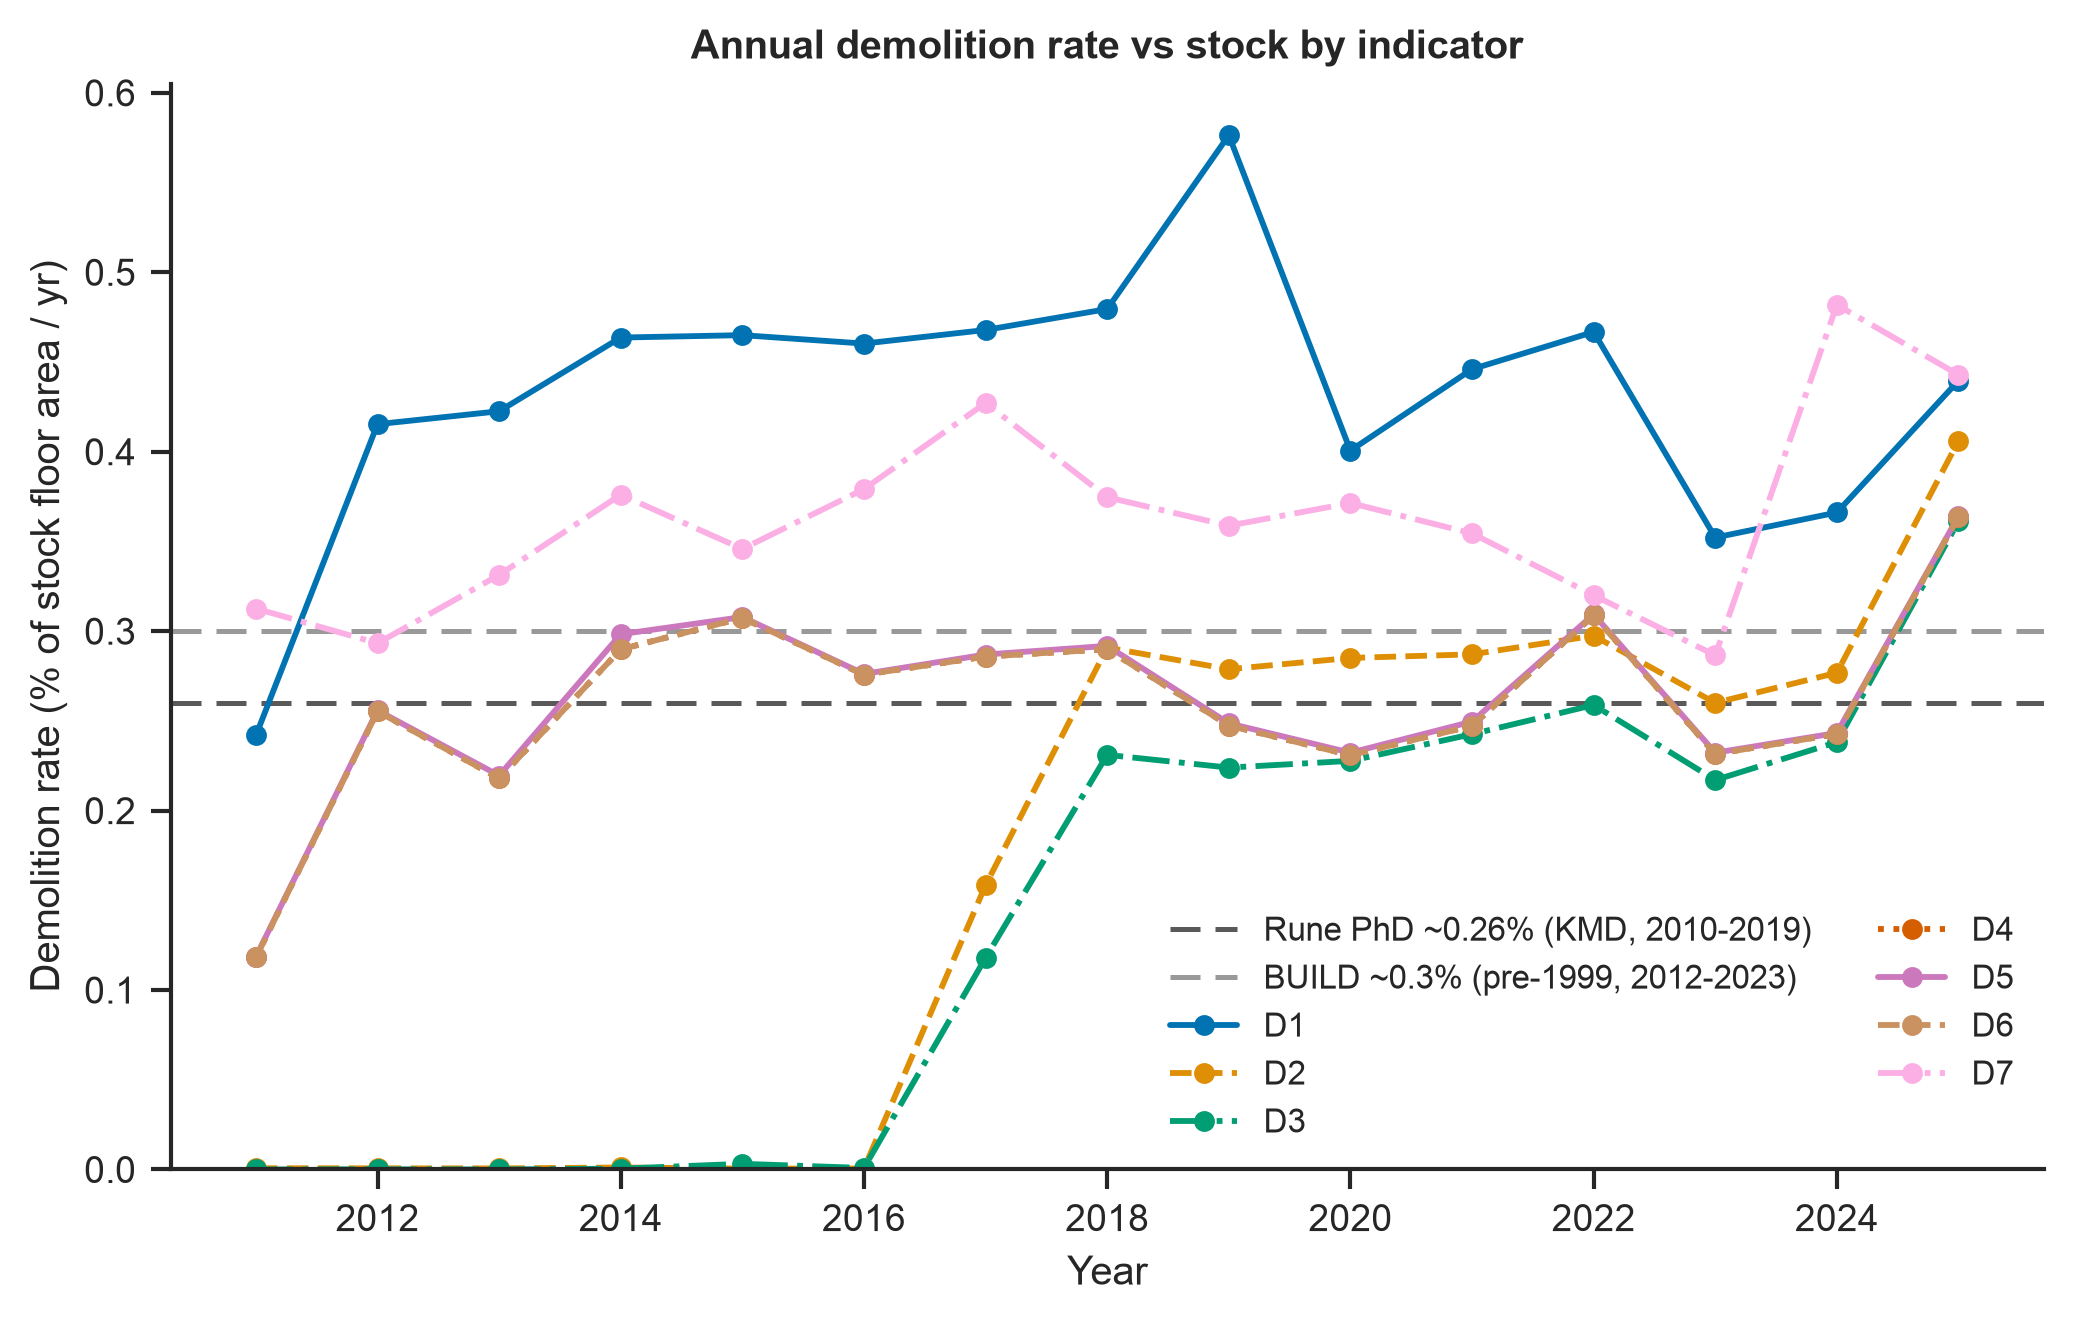
\includegraphics[width=0.7\textwidth]{media/rate_vs_stock.png}
\caption{Annual demolition rate per indicator, 2011--2025: complete-case
demolished residential-plus-commercial floor area divided by the matched
BYGB34 stock at 1~January of each year. D4 is hidden beneath D5 (their
dated annual series are identical). Dashed horizontal lines mark the
reference levels of 0.26 and 0.3\,\% per year used for the comparison
with published estimates (Section~\ref{sec:build-comparison}).}
\label{fig:rate-vs-stock}
\end{figure}

\subsection{Comparison with published rate estimates}\label{sec:build-comparison}
%% STATUS: WRITTEN 2026-07-12 from rates_summary.csv (windows 2011-2019
%%   and 2012-2023) + the published PDFs on file. Was "Comparison with
%%   BUILD"; retitled because it now also carries the KMD-based published
%%   rate. BUILD's published reference numbers (verified against the
%%   report): ~26.6 M m2 retired 2012-2023 (pre-1999 buildings) ~= 2.2 M
%%   m2/yr ~= 0.3% of 674 M m2 stock; agriculture 46% of retired area.
%% NOTE (group): the ~0.26%/yr (2010-2019) level drawn in the figure is
%%   from Rune Andersen's PhD thesis (DTU 2023), which has NO entry in
%%   references.bib — hence the \refneeded below. The citable published
%%   figure from the same extract is 0.24% (2011-2019, annual range
%%   0.20-0.28%) in \cite{andersen2022adaptation} (verified against the
%%   PDF on file, §5.1 and §6).
The published national demolition rate computed from the KMD extract of
Section~\ref{sec:kmd} is an average of 0.24\,\% of the existing
building-stock floor area per year over 2011--2019, with annual values
between 0.20 and 0.28\,\%~\cite{andersen2022adaptation}. Over the same
window, the primary pairing gives 0.254\,\% per year for D4 and D5: the
total-demolition-case family that Section~\ref{sec:kmd} shows coincides
with the extract also lands inside the published annual range. The
remaining indicators fall outside it --- D1 at 0.444\,\%, and D2 and D3 at
0.081\,\% and 0.064\,\%, the last two pulled down by their near-empty
pre-2016 series (Section~\ref{sec:rate-vs-stock}); the notification-dated
D6 \pending{recompute the D6 rate with src/rates.py after the total-only
redefinition}. A closely related KMD-based figure of
approximately 0.26\,\% per year over 2010--2019 \refneeded{Rune Andersen
PhD thesis (DTU 2023); add verified entry before citing} is drawn as a
reference level in Figure~\ref{fig:rate-vs-stock}; BYGB34 begins in
2011, so its 2010 start year cannot be matched here.

BUILD's analysis counts buildings constructed before 1999 that were
retired (``udg{\aa}et'') from the register in 2012--2023 and reports
approximately 26.6~million~m\textsuperscript{2} of retired
residential-plus-commercial floor area over those twelve years --- about
2.2~million~m\textsuperscript{2} per year, or 0.3\,\% of a
674~million~m\textsuperscript{2} stock on the same area
basis~\cite{jensen2025nedrivning}. We do not apply their construction-year
restriction, so over 2012--2023 our numerator is wider than theirs. On
that window the primary pairing runs from 0.127\,\% per year (D3) to
0.451\,\% (D1), with the total-demolition-case indicators D4/D5 at
0.266\,\% and D2 at 0.155\,\% (D6 \pending{recompute}); BUILD's
approximately 0.3\,\% lies inside this band. In absolute terms the same
window gives 0.9--3.0~million~m\textsuperscript{2} per year across the
indicators (case family 1.8), around BUILD's approximately
2.2~million~m\textsuperscript{2} per year.
\groupdecision{Methods Section~\ref{sec:comparisons} still announces a
reproduction of BUILD's exact setup (pre-1999 buildings only); the
comparison above applies no construction-year cut (decided 2026-07-12).
Align the Methods text, or decide whether the exact-setup run is still
wanted.}

%% =========================================================================
\section{Discussion}\label{sec:discussion}

\draftnote{Outline only --- to be written by the group from the results.
The topic list follows our planning documents (plan.md \S2, \S10--11);
no positions are taken in this draft.}

%% Planned discussion topics (from the research questions and the
%% interpretation framework in docs/plan.md):
%%
%%  1. Pros and cons of each indicator, in light of the results:
%%     - overlap/disagreement patterns (which buildings, how much area);
%%     - failure modes observed per indicator (reactivations, missing
%%       process codes, discontinued-code concentration, migration-era
%%       artifacts);
%%     - the interpretation framework of plan.md §10 (high-confidence /
%%       likely / activity-unclear / ambiguous / inconsistent /
%%       unresolved) applied to the findings.
%%  2. Pros and cons of each area measure (completeness vs. concept;
%%     what the byg038 missingness structure implies; what the BUILD
%%     reconstruction shows about comparability).
%%  3. Comparison with published estimates: BUILD's udgået-based totals
%%     (incl. their own caveats and pre-1999 filter), the 0.3 %/yr
%%     cost-statistics rate, and the survival-analysis service lives.
%%     [Numbers and reading: group, after results.]
%%  4. Whether the results support recommendations for BBR-based
%%     research, and which (plan.md §11 sketches candidate wording).
%%  5. Limitations: registration-history floor (2017), self-reporting,
%%     no national ground truth, partial demolitions, generalizability.
%%
%% TODO (group): write 5.1-5.5 from the above once results/ is populated.

\slotfor{RUNE / NICOLAI --- framing}{Positioning of the findings in the
international literature and their implications beyond Denmark; connects
to the related-work slot in the Introduction.}

%% =========================================================================
\section{Conclusion}\label{sec:conclusion}
%% TODO (group): 3-4 paragraphs max; mirror the abstract's claims.
%% Write last.
\pending{conclusion --- written by the group once results and discussion
are settled}

%% =========================================================================
%% Declarations required by JOBE
%% =========================================================================

\section*{CRediT authorship contribution statement}
%% TODO: fill per author once the author list and order are decided.
%% (JOBE requires CRediT roles; no authorship changes after acceptance.)
\groupdecision{author list, order, corresponding author, and CRediT
roles}

\section*{Declaration of competing interest}
The authors declare that they have no known competing financial interests
or personal relationships that could have appeared to influence the work
reported in this paper.

\section*{Funding}
This research did not receive any specific grant from funding agencies in
the public, commercial, or not-for-profit sectors.

\section*{Data availability}\label{sec:data-availability}
%% TODO: finalize once the dataset is deposited (planned: demolitions.parquet
%% + analysis code from the bbr-demolitions repo, e.g. Zenodo/DTU Data).
The cleaned analysis dataset and analysis code supporting this study are
openly available at \pending{repository DOI --- planned deposit}. The
underlying register data are publicly available from the Danish Data
Distributor (Datafordeler).

\section*{Declaration of generative AI and AI-assisted technologies in the manuscript preparation process}
%% DRAFT wording — keep the tool list updated as work proceeds.
During the preparation of this work the authors used large language model
assistants (Anthropic Claude) in order to edit manuscript text and assist
with bibliographic verification and analysis code. After using these
tools, the authors reviewed and edited the content as needed and take
full responsibility for the content of the published article.

\section*{Acknowledgements}
%% TODO: acknowledge Nicolai Siim Larsen / Rune Andersen here ONLY IF they
%% are not co-authors (never both acknowledge and author the same person).


%% =========================================================================
\bibliographystyle{elsarticle-num}
\bibliography{references}

%% =========================================================================
%% \appendix
%% \section{Full code lists}  — TODO: complete Livscyklus /
%%   ForretningsProcess / case-type lists with access date, if the group
%%   wants them in the paper (source: \cite{bbr_kodelister}).
%% \section{Lifecycle-history patterns} — plan.md suggests additional
%%   lifecycle plots go in an appendix.

\end{document}
